% !TEX root = thesis.tex
\documentclass[12pt,a4paper,titlepage,listof=totoc,bibliography=totoc,chapteratlists=0pt]{scrreprt}
\begin{filecontents*}{\jobname.xmpdata}
	\Keywords{CHANGEME, VR, IOT, TODO}
	\Title{Relaxoon}
	\Author{Abdulrahman Al Sabagh, Moritz Eder}
\end{filecontents*}

\setcounter{tocdepth}{1}

\usepackage[utf8]{inputenc}
\usepackage[T1]{fontenc}
\usepackage{amsmath}
\usepackage{amsfonts}
\usepackage{amssymb}
\usepackage[table]{xcolor}
\usepackage{graphicx}
\usepackage[left=3.50cm, right=2.00cm, top=2.00cm, bottom=2.00cm,foot=1cm]{geometry}
\usepackage[splitrule,hang,flushmargin,multiple,bottom]{footmisc}
\usepackage{lmodern, textcomp}
\usepackage{lmodern}
\usepackage{pdfpages}
\usepackage[ngerman]{babel}
\usepackage{multicol}
\usepackage{float}
\usepackage{array,tabularx,booktabs}
\usepackage{ragged2e}
\usepackage{lipsum}
\usepackage{wrapfig}

\newcolumntype{M}[1]{>{\centering\arraybackslash}m{#1}}

\usepackage{enumitem}
\newlist{compactitem}{itemize}{3}
\setlist[compactitem,1]{label=\textbullet, nosep,leftmargin=1.5em,labelwidth=*,align=left}
\setlist[compactitem,2]{label=--, nosep,leftmargin=1.5em,labelwidth=*,align=left}
\setlist[compactitem,3]{label=\textopenbullet, nosep,leftmargin=1.5em,labelwidth=*,align=left}
\newlist{compactenum}{enumerate}{3}
\setlist[compactenum,1]{label=\arabic*., nosep,leftmargin=1.5em,labelwidth=*,align=left}
\setlist[compactenum,2]{label=\alph*., nosep,leftmargin=1.5em,labelwidth=*,align=left}
\setlist[compactenum,3]{label=\roman*., nosep,leftmargin=1.5em,labelwidth=*,align=left}
\newlist{compactdesc}{description}{3}
\setlist[compactdesc]{leftmargin=1.5em,labelwidth=*,align=left}

\usepackage{microtype}

\usepackage[parfill]{parskip}

\definecolor{bluekeywords}{rgb}{0.13,0.13,1}
\definecolor{greencomments}{rgb}{0,0.5,0}
\definecolor{redstrings}{rgb}{0.9,0,0}
\definecolor{lightgray}{gray}{0.9}
\definecolor{lightblue}{rgb}{0.93,0.95,1.0}

\usepackage{listings}

\makeatletter
\lstdefinestyle{lststyle}{
	basicstyle=%
	\ttfamily
	\lst@ifdisplaystyle\scriptsize\fi
}
\makeatother

\renewcommand{\lstlistlistingname}{List of Listings}
% TODO: define other languages as needed
\lstset{language=Python,
	numbers=left,
	numberstyle=\tiny,
	showspaces=false,
	showtabs=false,
	breaklines=true,
	lineskip=-1pt,
	tabsize=2,
	showstringspaces=false,
	breakatwhitespace=true,
	escapeinside={(*@}{@*)},
	commentstyle=\color{greencomments},
	keywordstyle=\color{bluekeywords}\bfseries,
	stringstyle=\color{redstrings},
	style=lststyle,
	xleftmargin=17pt,
	framexleftmargin=17pt,
	framexrightmargin=5pt,
	framexbottommargin=4pt
}
\lstset{
	morekeywords={base,var,in,out,dynamic,from,where,select,orderby,function,\$,group,by,into,yield,async,await,@,None,self,as,elif,with}
}
\lstdefinelanguage{TypeScript}{
	keywords={typeof, new, true, false, catch, function, return, null, switch, var, if, in, while, do, else, case, break, void, number, string, boolean, module, \$, export, for, this},
	keywordstyle=\color{blue}\bfseries,
	ndkeywords={class, export, boolean, throw, implements, import, this},
	ndkeywordstyle=\color{darkgray}\bfseries,
	identifierstyle=\color{black},
	sensitive=false,
	comment=[l]{//},
	morecomment=[s]{/*}{*/},
	commentstyle=\color{purple}\ttfamily,
	stringstyle=\color{red}\ttfamily,
	morestring=[b]',
	morestring=[b]"
}
\usepackage{caption}
\DeclareCaptionFont{white}{\color{white}}
\DeclareCaptionFormat{listing}{\colorbox[cmyk]{0.43, 0.35, 0.35,0.01}{\parbox{\textwidth}{\hspace{10pt}#1#2#3}}}
\captionsetup[lstlisting]{format=listing,labelfont=white,textfont=white}
\captionsetup[table]{justification=centering, singlelinecheck=false}

\usepackage{subcaption}

\usepackage{setspace}
\newcommand{\MSonehalfspacing}{%
	\setstretch{1.44}%  default
	\ifcase \@ptsize \relax % 10pt
		\setstretch {1.448}%
	\or % 11pt
		\setstretch {1.399}%
	\or % 12pt
		\setstretch {1.433}%
	\fi
}

\newcommand{\setauthor}[1]{\ohead[]{#1}}

\usepackage[automark]{scrlayer-scrpage}
\pagestyle{scrheadings}
\automark{chapter}
\renewcommand\sectionmark[1]{\markright{\MakeMarkcase {\thesection\hskip .5em\relax#1}}}
\rohead{\ifnum\expandafter\pdfstrcmp\botmark=0 \rightmark\else\leftmark{} --- \rightmark\fi}
\ihead[]{\headmark}
\chead[]{}
\ohead{}
\cfoot[]{}
\ofoot[\pagemark]{\pagemark}
\setheadsepline{.1pt}

\usepackage[hyphens]{url}

\usepackage[a-1b]{pdfx}

\usepackage{hyperref}
\hypersetup{pdfa}

\usepackage[nonumberlist,toc,nopostdot]{glossaries}

\usepackage{chngcntr}
\counterwithout{footnote}{chapter}
\counterwithout{figure}{chapter}
\counterwithout{table}{chapter}
\AtBeginDocument{
	\counterwithout{lstlisting}{chapter}
	\urlstyle{sf}
}
\newcounter{RPages}

\makeatletter
\def\bstctlcite{\@ifnextchar[{\@bstctlcite}{\@bstctlcite[@auxout]}}
\def\@bstctlcite[#1]#2{\@bsphack
	\@for\@citeb:=#2\do{%
		\edef\@citeb{\expandafter\@firstofone\@citeb}%
		\if@filesw\immediate\write\csname #1\endcsname{\string\citation{\@citeb}}\fi}%
	\@esphack}
\makeatother

\clubpenalty=10000 
\widowpenalty=10000
\displaywidowpenalty=10000
\interfootnotelinepenalty=10000

\title{Relaxoon}
\author{Abdulrahman Al Sabagh, Moritz Eder}

\makeindex
\makeglossaries
\begin{document}
\bstctlcite{IEEEexample:BSTcontrol}
\newcommand{\reminder}[1]
{ \textcolor{red}{<[{\bf\marginpar{\mbox{$<==$}} #1 }]>} }
\newcommand{\icode}[1]{\lstinline$#1$}
%\urlstyle{same}
%\setstretch{1.5}
\setstretch {1.433}
\renewcommand{\arraystretch}{1.2}


\includepdf{./titlepage/coversheet}
\pagenumbering{Roman}
\newpage
\thispagestyle{empty}
\vspace{3cm}
~ \\ \\
Ich erkläre an Eides statt, dass ich die vorliegende Diplomarbeit selbstständig und ohne fremde Hilfe verfasst, andere als die angegebenen Quellen und Hilfsmittel nicht benutzt bzw. die wörtlich oder sinngemäß entnommenen Stellen als solche kenntlich gemacht habe.

Die Arbeit wurde bisher in gleicher oder ähnlicher Weise keiner anderen Prüfungsbehörde vorgelegt und auch noch nicht veröffentlicht.

Die vorliegende Diplomarbeit ist mit dem elektronisch übermittelten Textdokument identisch.
\vspace{3cm}
% Hier kommt die Unterschrift drüber
\begin{tabbing}
    Leonding, April 2024 \hspace{5cm} Abdulrahman Al Sabagh \& Moritz Eder
\end{tabbing}
\vspace{10cm}
\newpage
\setcounter{page}{1}

\setauthor{Moritz Eder}
\begin{spacing}{1}
    \chapter*{Abstract}
\end{spacing}
\begin{wrapfigure}{r}{0.3\textwidth}
    \begin{center}
      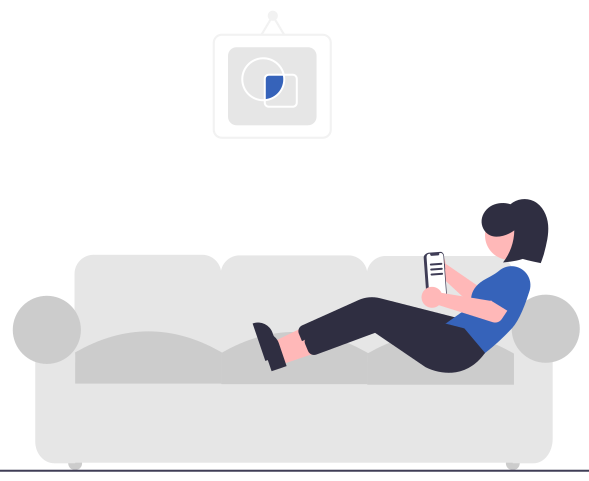
\includegraphics[width=0.3\textwidth]{pics/undraw_Relaxing_at_home_re_mror.png}
    \end{center}
\end{wrapfigure}
In order to give stressed people a simple way to relax, a stress management app has been developed.

Relaxoon is a play on the words 'relax' and 'soon'. Relaxoon offers relaxation exercises in the form of videos, 
texts, articles and more, which are presented in a simple and clear way.

In addition to implementing the front end in React Native and the back end with the content management system
Strapi, the deployment using Kubernetes is described in detail.
\newpage
\begin{spacing}{1}
    \chapter*{Zusammenfassung}
\end{spacing}
\begin{wrapfigure}{r}{0.3\textwidth}
    \begin{center}
      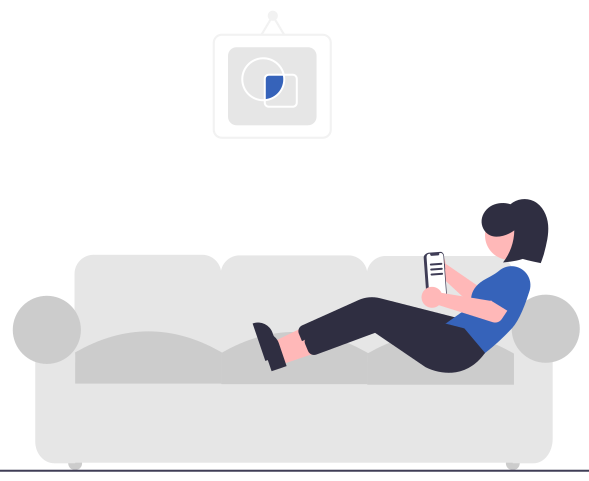
\includegraphics[width=0.3\textwidth]{pics/undraw_Relaxing_at_home_re_mror.png}
    \end{center}
\end{wrapfigure}
Damit gestresste Personen eine simple Möglichkeit haben, sich zu entspannen, wurde eine App zur Stressbewältigung
entwickelt. 

Relaxoon ist ein Wortspiel aus den englischen Wörtern 'relax' und 'soon'. Relaxoon bietet Entspannungsübungen 
in Form von Videos, Texten, Artikeln und mehr, die in einfacher und übersichtlicher Weise dargestellt sind.

Neben der Implementierung des Frontends in React Native und des Backends mit dem Content-Management-System
Strapi wird auf das Deployment mittels Kubernetes im Detail eingegangen.



\pagestyle{plain}

\renewcommand{\lstlistlistingname}{Quellcodeverzeichnis}

\tableofcontents
\newpage
\setcounter{RPages}{\value{page}}
\setcounter{page}{0}
\pagenumbering{arabic}
\pagestyle{scrheadings}

\begin{spacing}{1}
    \chapter{Abstract}\label{chapter:introduction}
\end{spacing}
\setauthor{Moritz Eder}
\begin{spacing}{1}
    \chapter*{Abstract}
\end{spacing}
\begin{wrapfigure}{r}{0.3\textwidth}
    \begin{center}
      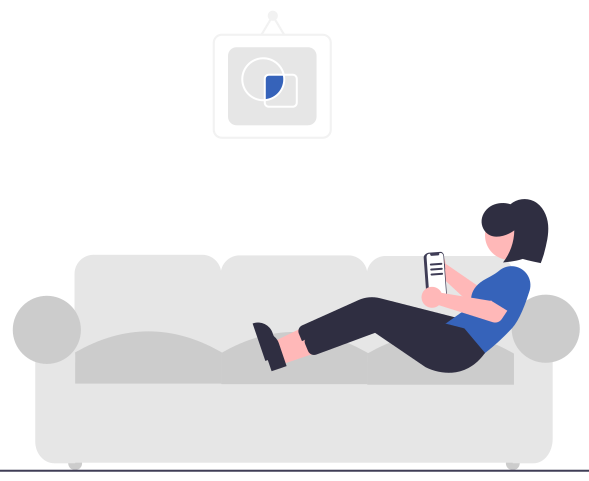
\includegraphics[width=0.3\textwidth]{pics/undraw_Relaxing_at_home_re_mror.png}
    \end{center}
\end{wrapfigure}
In order to give stressed people a simple way to relax, a stress management app has been developed.

Relaxoon is a play on the words 'relax' and 'soon'. Relaxoon offers relaxation exercises in the form of videos, 
texts, articles and more, which are presented in a simple and clear way.

In addition to implementing the front end in React Native and the back end with the content management system
Strapi, the deployment using Kubernetes is described in detail.
\newpage
\begin{spacing}{1}
    \chapter*{Zusammenfassung}
\end{spacing}
\begin{wrapfigure}{r}{0.3\textwidth}
    \begin{center}
      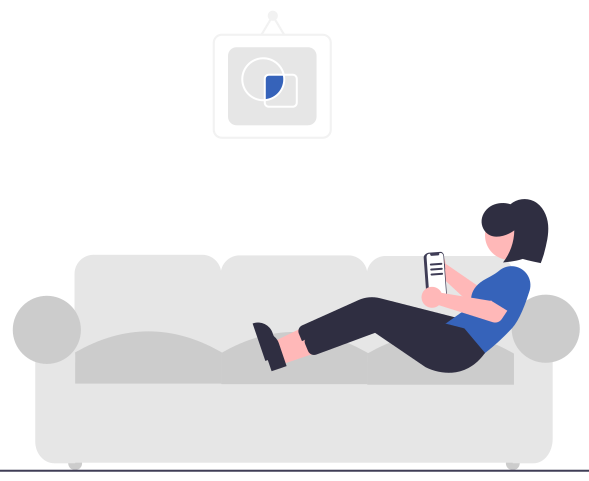
\includegraphics[width=0.3\textwidth]{pics/undraw_Relaxing_at_home_re_mror.png}
    \end{center}
\end{wrapfigure}
Damit gestresste Personen eine simple Möglichkeit haben, sich zu entspannen, wurde eine App zur Stressbewältigung
entwickelt. 

Relaxoon ist ein Wortspiel aus den englischen Wörtern 'relax' und 'soon'. Relaxoon bietet Entspannungsübungen 
in Form von Videos, Texten, Artikeln und mehr, die in einfacher und übersichtlicher Weise dargestellt sind.

Neben der Implementierung des Frontends in React Native und des Backends mit dem Content-Management-System
Strapi wird auf das Deployment mittels Kubernetes im Detail eingegangen.



\begin{spacing}{1}
    \chapter{Ausgangsituation}
\end{spacing}
\setauthor{Moritz Eder}

Heutzutage gibt es Stresssituationen, die dazu führen können, dass man manchmal den Überblick über die 
eigenen Aufgaben verliert. Um auch auf lange Zeit und produktiv Aufgaben erfüllen zu können, ist es sehr 
wichtig, dass man Ruhe und Entspannungsphasen in den Alltag einbaut, sei es in der Schule, der Universität
oder in der Arbeit. 

Langes und hartes Arbeiten kann zu zahlreichen gesundheitlichen Folgen führen, wobei Stress und 
Leistungsdruck das noch zusätzlich verschlimmern können. Eine häufige Konsequenz ist zum Beispiel
ein Burnout. Gemäß einer repräsentativen Studie aus dem Jahr 2016/17 fühlen sich nur 52 Prozent der 
Österreicher:innen tatsächlich gesund. 19 Prozent der Proband:innen befinden sich bereits in einem 
Burnout-Frühstadium, 17 Prozent sogar in einem Übergangsstadium. Schließlich ergab diese Studie, dass 
8 Prozent der Österreicher:innen unter dem Burnout-Syndrom leiden. \cite{burnout}

Deshalb greifen viele Menschen
auf die Musik zurück, wodurch sie sich beim Arbeiten entweder besser konzentrieren oder kurz
eine Pause einlegen können.

Zur Stressbewältigung wurde von der MACOLUTION GmbH und dem Data Science Unternehmen solvistas GmbH
eine Lösung für dieses Problem entwickelt. 
Die MACOLUTION GmbH ist ein Unternehmen, welches es sich zur Aufgabe gemacht hat,
Management- und Coaching-Solutions mit modernsten Technologien und bewährten Methoden zu entwickeln.
\cite{MACOLUTION}
Mit Relaxoon soll diese Idee Wirklichkeit werden.

\begin{figure}[H]
    \hspace{-2cm}
    \begin{minipage}{0.5\textwidth}
        \centering
        
\includegraphics[height=0.4\textwidth]{./pics/Logo-Macolution.jpg}
        \caption{Logo MACOLUTION}
    \end{minipage}
    \begin{minipage}{0.5\textwidth}
        \centering
        
\includegraphics[height=0.4\textwidth]{./pics/Logo-Solvistas.jpg}
        \caption{Logo solvistas}
    \end{minipage}
\end{figure}


\begin{spacing}{1}
    \chapter{Problemstellung}
\end{spacing}
\setauthor{Moritz Eder}

In der heutigen Welt entstehen immer mehr Termine für Besprechungen oder Meetings. 
Dadurch wird der generelle Alltag hektischer und schneller, was sowohl oft im Arbeitsleben als auch im 
privaten Bereich zutrifft. Daher empfinden viele Menschen den Ablauf des Tages persönlich als stressig.

Es fehlt außerdem die Möglichkeit sich zu entspannen und die Betroffenen verlieren den Mut sich
Hilfe zu holen.

Stress oder Leistungsdruck kann neben einem Burnout auch noch weitere gesundheitliche Folgen hervorrufen.
Mögliche Folgen von hohem Stress oder hohem Leistungsdruck können sein:

\begin{itemize}
    \item Zeichen von Nervosität
    \item Verspannungen, die zu Kopf-, Genick- und Rückenschmerzen führen können
    \item Vergesslichkeit
    \item Depressionen
    \item Psychische Störungen
\end{itemize}

Anhaltender Stress kann auch zu dauerhaften Herz/Kreislauf- und Nierenerkrankungen, Stoffwechselstörungen, 
Allergien oder Entzündungskrankheiten führen. \cite{stress} 
Gesundheit ist ein sehr wichtiger Faktor, deswegen benötigen gestresste Menschen eine Möglichkeit sich
wieder entspannen zu können.

\begin{figure}[H]
    \centering
    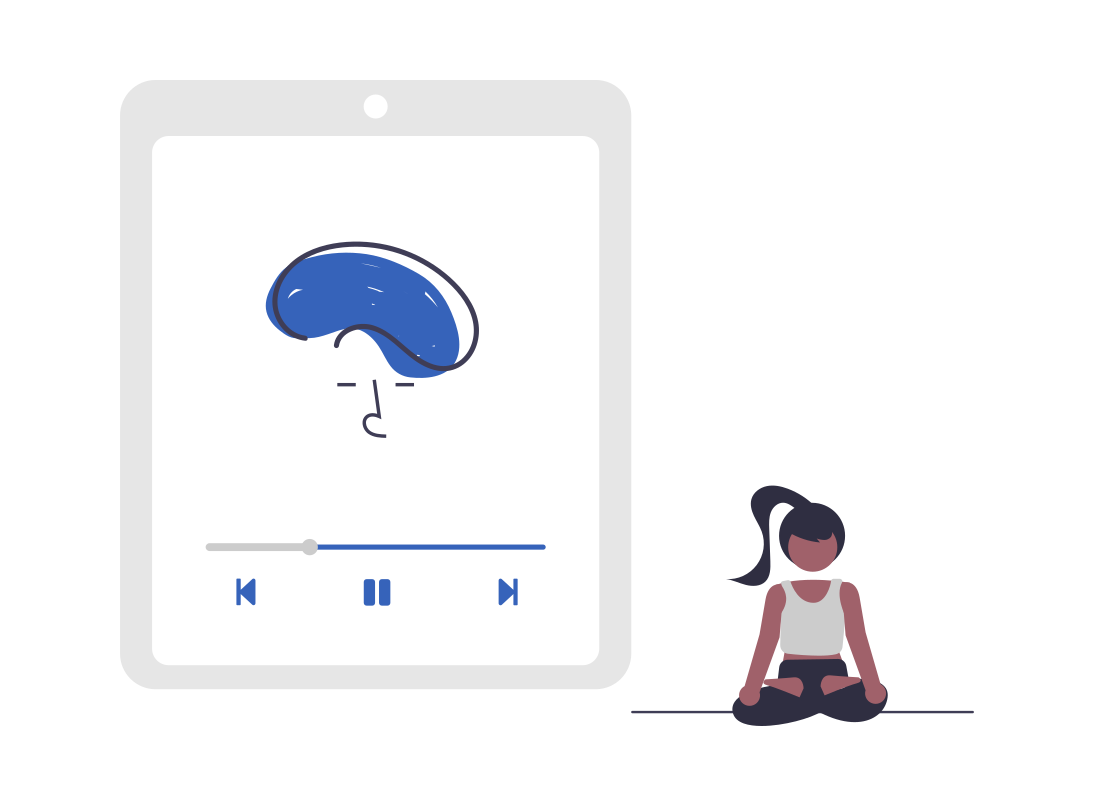
\includegraphics[height=0.35\textwidth]{./pics/undraw_Meditating_re_aiqa.png}
    \caption{Musik dient zur Entspannung}
\end{figure}



\begin{spacing}{1}
    \chapter{Ziele}
\end{spacing}
\setauthor{Moritz Eder}

Es gibt einen klaren Unterschiedzwischen dem Setzen von Zielen und dem tatsächlichen Erreichen von Zielen.
Das einfache Festlegen von Zielen allein genügt nicht. Um Erfolg in einem bestimmten Vorhaben zu haben,
ist es notwendig, klare Ziele zu definieren. Ein Ziel repräsentiert einen Zustand, ein Ergebnis oder einen
bestimmten Ort. Der Grad und die Art der Zielerreichung sind entscheidend für die Definition von Erfolg. Daher
ist das Festlegen eines Ziels lediglich der Ausgangspunkt. Dafür müssen Fortschritte oder Meilensteine
erreicht und der vorgegebene Zeitrahmen eingehalten werden – und dies alles unter Verwendung legaler und
legitimer Mittel und Methoden. Oftmals scheitert man nicht an mangelnder Disziplin oder Motivation, sondern
an falsch formulierten oder unpassenden Zielen.

Zielen charakterisieren sich durch einfache Aufgaben, die nach der Reihe erledigt werden – sie repräsentieren
feste Absichten. Hinter jedem Ziel steht immer ein konkretes Bestreben.
Ziele sind nicht nur das Ergebnis rationaler Überlegungen, sondern vor allem eine Angelegenheit des Herzens
und der Motivation.\cite{ziele}

\begin{figure}[H]
    \centering
    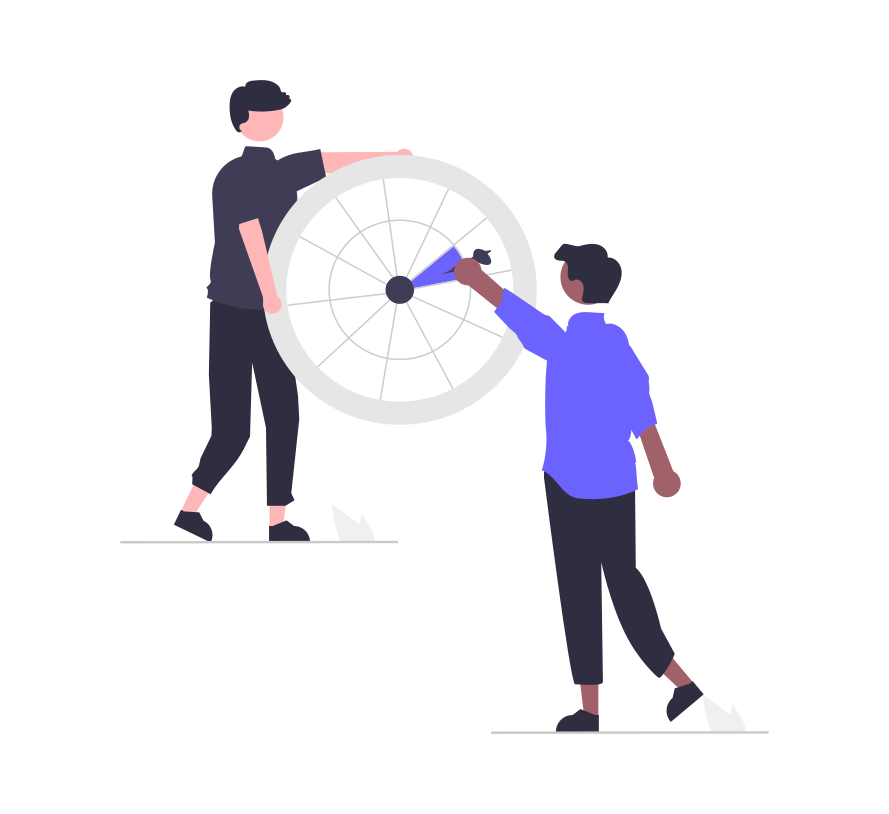
\includegraphics[height=0.45\textwidth]{./pics/undraw_Target_re_fi8j.png}
    \caption{}
\end{figure}

Ziele zu setzen ist wichtig, deswegen müssen sie von Anfang an \textbf{richtig} gesetzt werden. Beim Setzen der Ziele
kann man sich an folgenden Punkten orientieren: \cite{ziele}

\begin{itemize}
    \item Klare Konkretisierung ist entscheidend für Ziele! Je präziser die Beschreibung ist, desto einfacher
          ist es, darauf hinzuarbeiten.
    \item Ziele müssen realistisch sein! Zu ehrgeizige Ziele können Frustration und Selbstzweifel
          auslösen. Sowohl das angestrebte Ergebnis als auch die dafür vorgesehene Zeit sollten der Realität
          entsprechen.
    \item Wenn Ziele öffentlich gemacht werden, erhöht das auch die Erfolgswahrscheinlichkeit. Der Austausch
          über Ziele mit Familie, Freunden oder Kollegen steigert die Motivation und erzeugt Verbindlichkeit, da
          man es anderen beweisen möchte.
    \item Immer positiv bleiben! Positive Formulierungen der Ziele motivieren langfristig mehr.
    \item Ein eigener Antrieb ist notwendig, um die Zielabsicht vor Augen zu haben und um dranbleiben zu
          können.
    \item Ziele erfordern Flexibilität. Der Weg zum Ziel kann sich ändern, ebenso die Zeit für das Erreichen
          eines Meilensteins oder sogar das Ziel selbst. Ziele sind dynamisch und nie statisch oder unveränderlich.
    \item Zur Visualisierung der Ziele sollten sie stets in der Gegenwart formuliert werden, damit man sich
          gleich Bilder im Kopf vorstellen kann. Das steigert ebenso die Motivation.
\end{itemize}

\section{Projektziele}
Das Projekt soll zeigen, dass unter Verwendung des Open-Source headless CMS 'Strapi' und des mobilen 
React-Native Frontends einfach eine App zur Wiedergabe von Mediendateien für verschiedene mobile Betriebssysteme 
erstellt werden kann.

Ziel ist auch die Feinabstimmung der Qualität der Inhalte und wie diese optimal bereitgestellt werden können.
Wichtig ist dabei auch das für den Zweck passende Look and Feel.



\begin{spacing}{1}
    \chapter{Aufgabenstellung}
\end{spacing}
\setauthor{Moritz Eder}

Die Firma MACOLUTION hat Kontakte zu Streaming- und Gesundheitsexperten. Diese Fachleute erstellen viele Videos, 
Übungen und Artikel zu diesen Themen. Der Auftraggeber will eine Applikation für diese Kunden entwickeln, die folgende
Kriterien erfüllt:

\begin{itemize}
    \item User:innen müssen sich in der App nicht um die eigene Erstellung von Entspannungsmedien wie Texten oder Videos
    kümmern, weil diese Medien bereitgestellt werden, welche im Backend eingepflegt sind.
    \item Medien sollen
    individuell favorisierbar und mehreren Kategorien zugeteilt sein, die per Suchleiste in der App einfach zu
    finden sind.
\end{itemize}

Das Minimum Viable Product (MVP) von Relaxoon soll realisiert werden, damit möglichst früh Feedback von Nutzer:innen
eingeholt werden kann, welches für die Weiterentwicklung und für die Verbesserung der App essenziell ist.

Dies bestätigt der deutsche Content-Autor Philipp Steubel, der sich im amerikanischen Softwareunternehmen Asana
auf die Bereiche Marketing und 
Projektmanagement spezialisiert hat: "`Ein MVP ist sicherlich ein gutes Hilfsmittel, wenn es darum geht, den 
Entwicklungsprozess an den Kundenbedürfnissen zu orientieren. Immerhin bekommen Sie so schon während der 
Entwicklung des Produktes wertvolles Kundenfeedback. Somit erfahren Sie aber auch mehr über die Zielgruppe 
selbst, welche Personengruppen von dem Produkt bzw. dem Service überzeugt sind und wie Sie die Marketingkampagnen
aufsetzen können."' \cite{mvp}

% Personen, die oft gestresst vom Alltag sind, sollen durch Relaxoon wieder runterkommen
% und sich entspannen können, damit man sich wieder mit mehr Energie und einem klaren Kopf den
% nächsten Aufgaben stellen kann.

% Das Projekt soll zeigen, dass unter Verwendung des Open-Source headless CMS 'Strapi' und des mobilen
% React-Native Frontends eine App zur Wiedergabe von Mediendateien für verschiedene mobile Betriebssysteme
% und zur Stressbewältigung erstellt werden kann. 


% \begin{figure}[H]
%     \begin{minipage}{0.5\textwidth}
%         \centering
%         
\includegraphics[height=0.2\textwidth]{./pics/strapi-logo.png}
%         \caption{Logo Strapi}
%     \end{minipage}
%     \begin{minipage}{0.5\textwidth}
%         \centering
%         
\includegraphics[height=0.6\textwidth]{./pics/react-native-logo.png}
%         \caption{Logo React Native}
%     \end{minipage}
% \end{figure}

Wichtig dabei ist: 

\begin{itemize}
    \item die Feinabstimmung der Qualität der Inhalte
    \item die optimale Bereitstellung der sorgfältig ausgewählten Inhalte
    \item ein ansprechendes und benutzerfreundliches Design für den passenden ''Look and Feel'' der App.
\end{itemize}

\section{Use-Case-Diagram (UCD)}

Für Relaxoon gibt es im Wesentlichen zwei Hauptakteure: der/die Content-Manager:in und die Benutzer:innen der 
App. Diese Rollen interagieren mit verschiedenen Funktionen innerhalb der Anwendung, wie folgendermaßen 
dargestellt. Um die Übersichtlichkeit zu verbessern, wurde das UCD in zwei Teile aufgeteilt.

\begin{figure}[H]
    \centering
    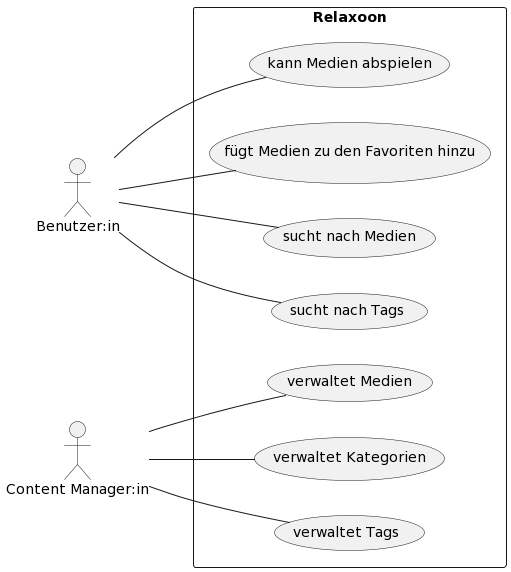
\includegraphics[height=\textwidth]{./pics/ucd1.png}
    \caption{Use-Case-Diagram 1}
\end{figure}

% @startuml

% left to right direction
% skinparam packageStyle rectangle

% actor "Benutzer:in" as Benutzer
% actor "Content Manager:in" as ContentManager

%     package "Relaxoon" {
%         usecase "kann Medien abspielen" as UC1
%         usecase "fügt Medien zu den Favoriten hinzu" as UC2
%         usecase "sucht nach Medien" as UC3
%         usecase "sucht nach Tags" as UC31
%         usecase "verwaltet Medien" as UC4
%         usecase "verwaltet Kategorien" as UC5
%         usecase "verwaltet Tags" as UC51
%     }

%     Benutzer -- UC1
%     Benutzer -- UC2
%     Benutzer -- UC3
%     Benutzer -- UC31
%     ContentManager -- UC4
%     ContentManager -- UC5
%     ContentManager -- UC51

% @enduml

\textbf{Benutzer:in}
\begin{itemize}
    \item kann Medien abspielen: kann vorhandene Medien in der Anwendung anzeigen, um sie anzusehen.
    \item fügt Medien zu den Favoriten hinzu: hat die Möglichkeit, bestimmte Medien als Favoriten zu markieren, um schnell auf sie zugreifen zu können.
    \item sucht nach Medien: kann in der Anwendung nach bestimmten Medien suchen, indem Suchkriterien eingegeben werden.
    \item sucht nach Tags: kann nach Medien suchen, indem nach bestimmten Tags oder Kategorien gefiltert wird, um gezielt Inhalte zu finden.
\end{itemize}
\textbf{Content Manager:in}
\begin{itemize}
    \item verwaltet Medien: kann Medien verwalten
    \item verwaltet Kategorien: kann Kategorien verwalten
    \item verwaltet Tags: kann Tags verwalten
\end{itemize}

\rule{\linewidth}{0.3pt}

Die Verwaltung der einzelnen Elemente wird im nächsten Diagramm genauer beschrieben.

\begin{figure}[H]
    \centering
    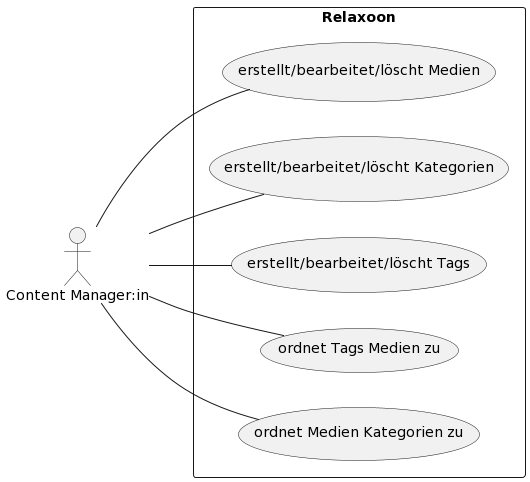
\includegraphics[height=0.84\textwidth]{./pics/ucd2.png}
    \caption{Use-Case-Diagram 2}
\end{figure}

% @startuml

% left to right direction
% skinparam packageStyle rectangle

% actor "Content Manager:in" as ContentManager

%     package "Relaxoon" {
%         usecase "erstellt/bearbeitet/löscht Medien" as UC4
%         usecase "erstellt/bearbeitet/löscht Kategorien" as UC5
%         usecase "erstellt/bearbeitet/löscht Tags" as UC51
%         usecase "ordnet Tags Medien zu" as UC81
%         usecase "ordnet Medien Kategorien zu" as UC8
%     }

%     ContentManager -- UC4
%     ContentManager -- UC5
%     ContentManager -- UC51
%     ContentManager -- UC8
%     ContentManager -- UC81

% @enduml

\newpage

\textbf{Content Manager:in}
\begin{itemize}
    \item erstellt/bearbeitet/löscht Medien: kann neue Medien in die Anwendung hochladen, vorhandene Medien bearbeiten und nicht mehr benötigte Medien entfernen.
    \item erstellt/bearbeitet/löscht Kategorien: kann neue Kategorien erstellen, bestehende Kategorien bearbeiten und überflüssige Kategorien löschen.
    \item erstellt/bearbeitet/löscht Tags: kann neue Tags erstellen, vorhandene Tags bearbeiten und ungenutzte Tags entfernen.
    \item ordnet Tags Medien zu: kann Tags bestimmten Medien zuweisen, um ihre Verschlagwortung und Klassifizierung zu optimieren.
    \item ordnet Medien Kategorien zu: kann Medien bestimmten Kategorien zuordnen, um ihre Einordnung und Auffindbarkeit in der Anwendung zu verbessern.
\end{itemize}


\begin{spacing}{1}
    \chapter{Systemarchitektur}\label{chapter:system-architecture}
\end{spacing}
\section{Komponentendiagramm}

Für eine klare funktionale Übersicht auf unserer Diplomarbeit
wurde ein sogenanntes Komponentendiagramm für das technische System von Relaxoon erstellt.
Da Relaxoon eine Applikation ist, die auf Handys laufen soll,
wurde für die Entwicklung die cross plattformige \textbf{J}ava\textbf{S}cript  (js)
Framework "React Native" verwendet. Damit der Kunde Inhalte in die App hinzufügen kann,
wurde ein "Node js" basiertes Headless \textbf{C}ontent \textbf{M}anagement \textbf{S}ystem (CMS)
namens “Strapi” verwendet.
Dieses bietet eine vorgefertigte Benutzeroberfläche für die Content Creators
und auch für die Entwickler, sodass man Inhalte und dazu gebrauchte technische Funktionalitäten, wie zum Beispiel
\textbf{RE}presentational \textbf{S}tate \textbf{T}ransfer (REST)- bzw. \textbf{G}raph \textbf{Q}uery \textbf{L}anguage (Graphql)-Schnittstellen
für die Authentifizierung und \textbf{C}reate, \textbf{R}ead, \textbf{U}pdate und \textbf{D}elete (CRUD)
Funktionalitäten jeder Business Entität, sehr einfach erstellen kann.
Für die Kommunikation zwischen Frontend und Backend wird REST verwendet. Das Backend holt sich die Daten mit Hilfe eines postgresql Treibers aus der Datenbank.


\begin{figure}[H]
    \centering
    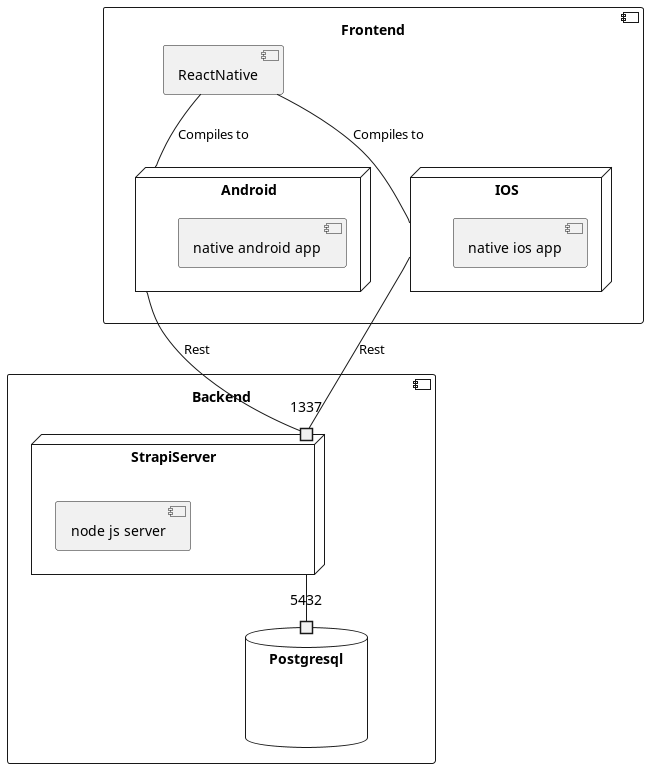
\includegraphics{./pics/system-architektur.png}
    \caption{Systemarchitektur}
    \label{fig:Systemarchitektur}
\end{figure}


\begin{spacing}{1}
    \chapter{Entwurfsentscheidungen}\label{chapter:Entwurfsentscheidungen}
\end{spacing}
\setauthor{Abdulrahman Al Sabagh}
\begin{spacing}{1}

    \section{React Native}

    Grundsätzlich wurde React Native aus mehreren Gründen verwendet:
    \begin{itemize}
        \item React Native ist das Standardframework für cross-plattform-Lösungen bei der Firma Solvistas.
        \item Vorhandene Kenntnisse in den Sprachen Javascript bzw. Typescript
        \item Auftraggber forderte eine cross-plattform-Lösung für das Frontend, um IOS- Android- Betriebssysteme abzudecken
        \item Endergebnis von React Native ist eine native App
    \end{itemize}




    \subsection{Was ist eine cross-plattform-Lösung}

    \begin{quotation}
        ``
        Eine Cross-Platform App besteht aus einem einzigen Code,
        der jeweils in die native Systemsprache von Apple, Android \& Co. kompiliert wird.
        Dadurch erhält man eine App, die mit wenig Entwicklungsaufwand auf mehreren
        Betriebssystemen zur Verfügung steht, sich aber dennoch wie eine native App
        anfühlt.''
        \cite{cross-plattform}

    \end{quotation}


    \subsection{Warum wurde eine cross-plattform-Lösung angefordert}
    Der Client von Relaxoon besteht aus einer einfachen Applikation, die keine Business Logik
    und auch keine Performance kritische Funktionalitäten hat.
    Daher ist die Verwendung einer cross-plattform-Lösung sehr vorteilhaft,
    da alle Plattformen von einem Codebase gepflegt werden können.



    \subsection{Warum ist Relaxoon native und nicht hybrid}

    \textbf{hybride Applikationen}: \begin{quotation}
        ``
        Eine hybride App kombiniert die besten Elemente von [N]ativen und Web-Apps.
        Sie werden wie eine native App installiert, aber es ist eigentlich
        eine Web-App innerhalb des Endgeräts.
        Hybride Apps werden in den gängigsten Sprachen für die Web-App Entwicklung, wie z.B. HTML und CSS, programmiert. Dies bedeutet, dass sie auf verschiedenen Plattformen verwendet werden können.
        Obwohl sie in der Sprache der Webanwendung entwickelt wurden, haben sie die gleiche Fähigkeit wie native Apps, sich an verschiedene Geräte, wie ein Tablet, Smartphone usw. anzupassen.
        ''
        \cite{native-vs-hybrid}
    \end{quotation}
    \textbf{natvie Applikationen}: \begin{quotation}
        ``
        Eine native App ist eine Anwendung, die entwickelt wurde,
        um auf einer bestimmten Plattform oder einem bestimmten Endgerät zu arbeiten.
        Aus diesem Grund können native Apps mit den auf der jeweiligen Plattform
        installierten Betriebssystem[s]funktionen interagieren und diese nutzen.
        ''

        \cite{native-vs-hybrid}

    \end{quotation}

    Grundsätzlich sind native Applikationen  viel schneller und barrierefreier als hybride Applikationen
    \cite{native-vs-hybrid}



    \subsection{Alternativen für React Native}

    \subsubsection{Kotlin Multiplatform}
    \textbf{K}otlin \textbf{M}utli\textbf{P}lattform (KMP) bietet bessere Performance als React Native und hat auch eine modulare Integration.
    \newline
    \textbf{modulare Integration}: \begin{quotation}
        ``
        Probably the biggest benefit in favor of Kotlin Multiplatform is that it’s
        an SDK and not a framework. This means that teams with existing apps can
        simply add a module or migrate a small part to assess its viability without
        a huge commitment. This really helps Kotlin address the biggest deterrent
        when moving to a new codebase.
        ''
        \cite{kotlin-multiplatform-vs-react-native}
    \end{quotation}
    Allerdings ist das Problem davon, dass KMP noch immer im Beta ist und daher ist diese nicht stabil.
    Außerdem  ist die Community von dieser Alternative nicht so groß wie die Community von React Native.
    Gute Kenntnisse in Swift \textbf{U}ser \textbf{I}nterface (UI) und Android \textbf{S}oftware \textbf{D}evelopment \textbf{K}it (SDK) werden für die Verwendung von Kotlin Multiplatform auch verlangt.
    Grund dafür ist, dass KMP keine Bilbiotheken für UI-Elementen wie React Native oder Flutter bereitstellt, sondern die Syntax der OS-Technologie verwendet.
    \cite{kotlin-multiplatform-vs-react-native}
    \subsubsection{Flutter}

    Flutter an sich ist viel schneller als React Native.
    Außerdem unterstüzt Flutter die Betriebssysteme  Windows, Linux und Macos zusätzlich zu Web, Android und IOS.
    \cite{flutter-vs-react-native}
    \newline
    Das Problem bei Flutter ist, dass man gute Kenntnisse in der Programmiersprache ''Dart'' haben muss. \cite{flutter-vs-react-native}
    Für die Entwicklung von React Native sind gute Kenntnisse in den Programmiersprachen Javascript und Typescript,
    die wir bereits gelernt haben,
    gebraucht.
    Außerdem ist die Unterstützung von Macos, Linux und Windows für uns gar nicht relevant.


    \subsubsection{Xamarin}

    Xamarin ist eine C\# Framework, die für die Entwicklung von nativen cross-plattform-Lösungen zuständig ist.
    Die Performance von Xamarin ist viel besser als die Performance von React Native. \cite{xamarin-vs-react-native}

    Die Entwickler haben sich aus den Gründen, die bei Flutter bereites erwähnt wurden, für React Native entschieden.
    Außerdem gibt es beim Xamarin kein ''hot reloading'' und daher muss das
    Program bei jeder kleinen Änderung neugestartet werden.\cite{xamarin-vs-react-native}



    \subsection{Nutzwertanalyse für das Frontend-Framework}
    \begin{tabular}{|p{5cm} | p{2cm} | p{2cm} | p{2cm} | p{2cm} | }
        \hline
        Kriterien                      & React Native & Xamarin & Flutter & KMP  \\
        \hline
        Vorhandene Kenntinsse max.50\% & 50\%         & 0\%     & 0\%     & 10\% \\
        \hline
        Barrierfreiheit max. 30\%      & 15\%         & 5\%     & 30\%    & 20\% \\
        \hline
        Performance max. 20\%          & 5\%          & 20\%    & 15\%    & 10\% \\
        \hline
        Summe                          & 70\%         & 25\%    & 45\%    & 40\% \\
        \hline
    \end{tabular}





    \section{Strapi}

    \subsection{Was ist ein CMS}

    \begin{quotation}
        ``Ein Content-Management-System (CMS) ist eine Softwareanwendung,
        die es Benutzern ermöglicht, digitale Inhalte zu erstellen, zu bearbeiten, gemeinsam zu editieren,
        zu veröffentlichen und zu speichern. Content-Management-Systeme werden typischerweise für Enterprise
        Content Management (ECM) und Web Content Management (WCM) eingesetzt.''
        \cite{cms}
    \end{quotation}



    \subsection{Warum wurde ein CMS verwendet}
    Der Auftragsgeber wollte die Applikation so schnell wie möglich veröffentlichen,
    da die Anzahl der Apps, welche die gleichen Anwendungsfälle wie Relaxoon haben,
    nicht so groß ist.
    Daher ist die Verwendung eines fertigen CMSes viel schneller als
    die Implementierung eines Backends.

    \subsection{Was ist ein Headless-CMS}
    \begin{quotation}

        ``
        Ein Headless CMS ist sowohl eine Weiterentwicklung als
        auch eine Verknappung eines klassischen CMS. Dem System
        werden integrale Bestandteile genommen, um es für
        unterschiedlichste Ausgaben kompatibel zu machen.
        Das gelingt dadurch, dass Frontend und Backend in einem
        Headless CMS nicht mehr monolithisch miteinander verknüpft
        sind. Das fehlende Frontend ist auch der Grund,
        wieso derartige CMS-Systeme als
        „kopflos“ (englisch: „headless“) bezeichnet werden.
        '' \cite{headles-cms}
    \end{quotation}

    \subsection{Warum wurde ein Headless-CMS verwendet}
    \begin{itemize}
        \item Vorgabe von dem Auftragsgeber
        \item Andere Arten von CMSes generieren statische HTML Seiten, welche für Relaxoon gar nicht gebraucht werden,
              da Relaxoon eine Mobileapp ist
        \item die Firma Solvistas beschäftigt sich intensiv mit Data Science. Da man auf dem CMS mittels REST zugreifen kann,
              will Solvistas ein Datenzentrum aus diesem in der Zukunft erstellen, zusätzlich zur Verwendung von CMS für Data Science Zwecke.
    \end{itemize}
    \subsection{Warum Strapi und nicht Wordpress \textbf{AP}plication \textbf{I}nterface (API)}



    \subsubsection{Vorteile von Wordpress API}

    \begin{itemize}
        \item Es gibt sehr viele Einstellungen und Features
        \item Unterstüzt \textbf{S}earch \textbf{E}ngine \textbf{O}ptimization (SEO)
        \item guter Community Support
        \item Einfach zu verwenden
    \end{itemize}
    \cite{strapi-vs-wordpress}

    \subsubsection{Nachteile von Wordpress API}
    \begin{itemize}
        \item  Limitierte Flexibilität, da viele Plugins und Addons kostenpflichtig sind.
              die kostenlose Verwendung von einigen Addons und Plugins ist limitiert.
        \item Ist nicht geeignet für eine Software mit großer Skalierung
        \item Wordpress wird von vielen Menschen verwendet und deshalb ist es für die Hacker nicht unrelevant
        \item Die Benutzeroberfläche davon ist nicht gut designt und deshalb ist die Verwendung davon meistens sehr verwirrend und unangenehm zu bedienen
    \end{itemize}
    \cite{strapi-vs-wordpress}

    \subsubsection{Vorteile von Strapi}

    Im Gegensatz zu Wordpress, kann man mit Strapi beliebig viele Plugins und Addons
    verwenden. Außerdem gibt es eine eingebaute Authentifizierung bzw. Autorisierungsfunktion
    zusätzlich zur Unterstützung von 20 unterschiedlichen Sprachen und REST
    bzw. Graphql APIS.
    \cite{strapi-vs-wordpress}

    \subsubsection{Nachteile von Strapi}
    Ein Grundwissen in der Programmierung ist erforderlich, wenn man sich für Strapi
    entscheidet. Außerdem ist es nicht so weit verbreitet wie Wordpress und somit ist die Anzahl
    der 3rd-party-Libraries, die man in Strapi einbetten kann, nicht so groß.
    \cite{strapi-vs-wordpress}

    \subsubsection{Ergebnis}
    Alle erwähnten Pros und Contras zeigen, dass  die \textbf{U}ser E\textbf{X}perience (UX)
    und die Skalierbarkeit von Strapi viel besser als Wordpress ist.
    Außerdem ist Strapi viel schneller als Wordpress,
    da Strapi in "Node js" geschrieben ist und Wordpress in "PHP"
    \cite{strapi-vs-wordpress}

    \subsection{Nutzwertanalyse für das Headless-CMS}

    \begin{tabular}{ |p{3cm}|p{3cm}|p{3cm}| }
        \hline
        Kriterien                   & Strapi & Wordpress API \\
        \hline
        Security max.30\%           & 30\%   & 15\%          \\
        \hline
        Anpassbar max. 30\%         & 30\%   & 15\%          \\
        \hline
        Community Support max. 30\% & 10\%   & 25\%          \\
        \hline
        Performance max. 10\%       & 10\%   & 5\%           \\
        \hline
        Summe                       & 80\%   & 65\%          \\
        \hline
    \end{tabular}


\end{spacing}

\section{Component Library}
Der Standardweg, um UI-Elementen in React Native zu stylen, is JSS. Diese ist eine Technologie, wo man \textbf{C}ascading \textbf{S}tyle \textbf{S}heet (CSS)
in Form von Javascript Objekten schreibt. Das Problem bei dieser Technologie liegt dabei,
dass viele CSS Attribute und Funktionen nicht dabei inkludiert sind. Es gibt auch außerdem spezifische OS-Einstellungen für Barrierfreiheit wie zum Beispiel die Einstellungen für Screenreaders,
die man bei der Entwicklung immer wieder vergessen kann.
Aus diesen Gründen hat sich das Team für die Verwendung von 'Native Base' entschieden.



\begin{spacing}{1}
    \chapter{Implementierung}\label{chapter:implementation}
\end{spacing}
\setauthor{Abdulrahman Al Sabagh}
\section{\textbf{E}ntity \textbf{R}elationship \textbf{D}iagram (ERD)}
\begin{spacing}{1}

  \begin{figure}[H]
    \centering
    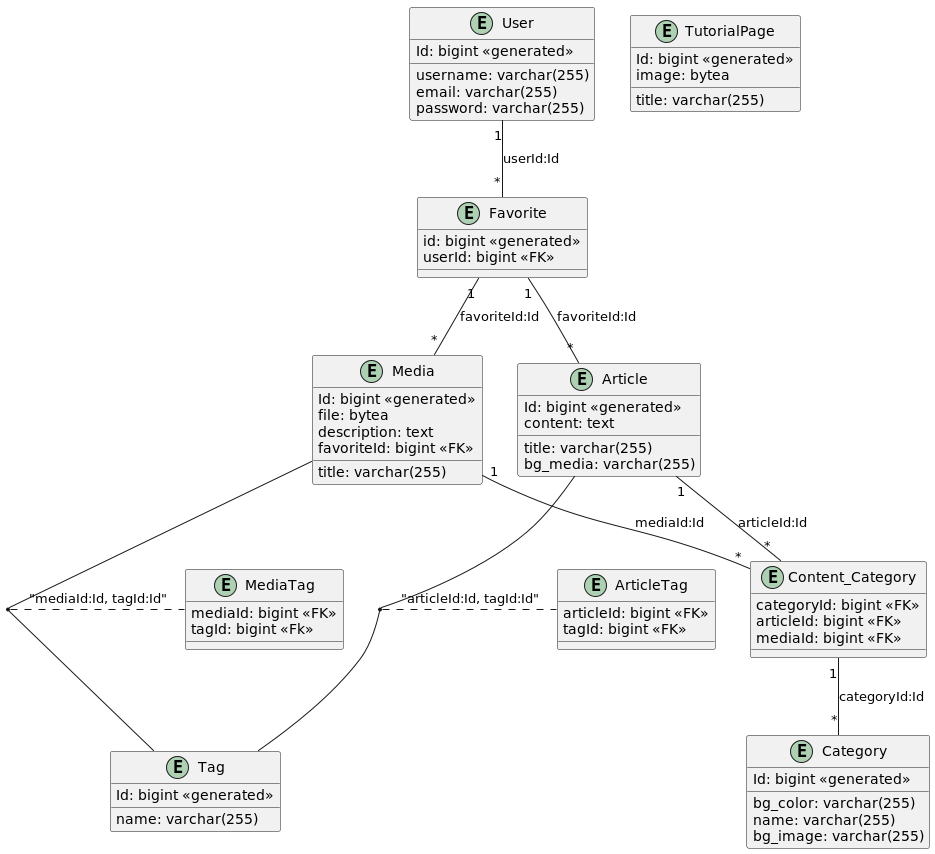
\includegraphics[height=1\textwidth]{./pics/erd.png}
    \caption{ERD}

  \end{figure}
\end{spacing}


\section{Medias und Articles}

Grundsätzlich wurde als Team entschieden,
die Artikel und die Medien in zwei seperaten Tabellen zu speichern,
da Artikel mehrere Bilder, Videos und Audios Inhalte enthalten können.
Diesen können dann mittels einem ''Rich Text Editor'' hinzugefügt werden.
Bei ''Media'' handelt es sich nur um ein Medienelement,
nämlich ein Bild, Video oder Audio File. Es ist aber wichtig anzumerken,
dass keine Benutzeroberfläche für die Artikel implementiert wurde, da der Kunde
diese nicht in dem \textbf{M}inimal \textbf{V}iable \textbf{P}roduct (MVP) haben wollte.
Für die Realisierung des kompletten Datenmodels war aber das Einfügen der Artikel erforderlich.

\section{TutorialPage}
Die Entität ''TutorialPage'' hat keine Beziehungen zu anderen Entitäten, da sie nur für den Inhalt des Tutorial-Slideshows,
die nach der erfolgreichen Installation der App angezeigt wird, gedacht ist.

\begin{figure}[H]
  \centering
  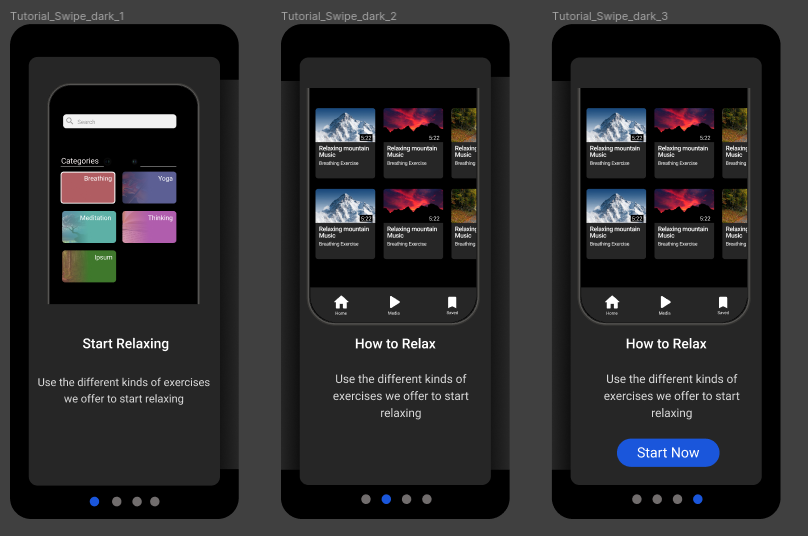
\includegraphics[height=0.5\textwidth]{./pics/slideshow.png}
  \caption{Screenshot aus dem UI Prototyp von Relaxoon}
\end{figure}

Mit dem Persistieren der Inhalte von der Slideshow könnte die Erstellung
von neuen Builds bei jeder Änderung vermieden werden.


\section{Suche und Filterungen}

Bei den Filterungen wurde der ''Interactive Query Builder'' verwendet,
um die Filterparameter der Abfragen zu generieren
und diese dann bei den REST Abfragen anzuhängen.
Es gibt auch eine ''Query Engine'', welche die gleiche Funktion wie diese
''Interactive Query Builder'' hat.
Diese kann in dem \textbf{O}bject \textbf{R}elational \textbf{M}apper (ORM) angewendet werden.
Mit der Verwendung dieser ''Interactive Query Builder'' kann man die Daten,
die man von den REST-Resourcen bekommt, anpassen.
Es gibt auch die Möglichkeit, die REST-Ressource im Backend mittels dieser
''Query Engine'' anzupassen.
Allerdings wurde diese ''Query Engine'' nicht verwendet,
da die Dokumentation bzw. IntelliSense von dem ORM sehr ungenau war.

\begin{figure}[H]
  \centering
  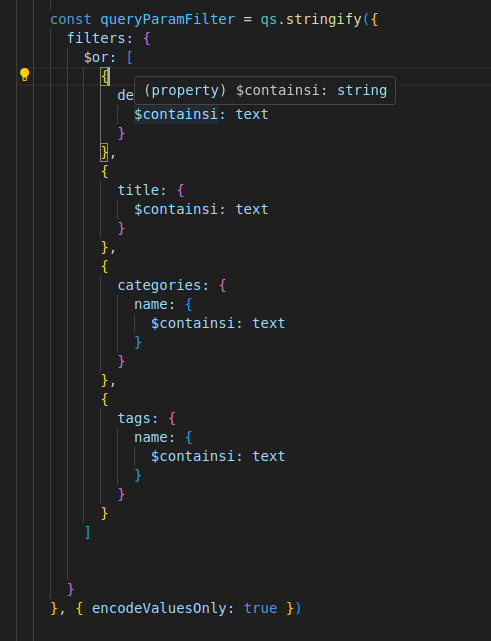
\includegraphics[ width=1\textwidth]{./pics/query-builder.png}
  \caption{Beispiel für den Interactive Query Builder}
\end{figure}




\begin{spacing}{1}
  \textbf{API-Route mit den angehängten generierten Abfrageparametern}:
  \newline
  \textcolor{red}{/medias?\&populate[tags]=true
  \&populate[file]=true
  \&populate[favorite][populate]=\newline users\_permissions\_user}
\end{spacing}


\section{State Management}
\begin{quotation}
  ``
  Der Begriff State ist in React-Applikationen überall präsent. Generell
  bezeichnet State den Zustand einer Komponente,
  also die dynamischen Daten, die eine Komponente den Benutzer:nnen anzeigt.
  Eine Änderung am State führt dazu, dass die Komponente neu gerendert wird
  und so die Datenänderung für die Benutzer:in sichtbar wird.
  Im einfachsten Fall verwaltet jede Komponente ihren eigenen State.
  Es gibt Fälle, in denen es jedoch erforderlich wird,
  den State zwischen mehreren Komponenten zu teilen.
  ''
  \cite{state-management}

  Um die Zustände der Applikation zu behandeln wurde meistens mit dem ''useState Hook'' von React gearbeitet.
  Der Einsatz einer State Management Library wie zum Beispiel ''RXJS'' oder ''Redux'' war gar nicht nötig, da die Anzahl der verwendeten UI-Komponenten nicht so groß ist.

  \subsection{useState Hook}
  ``useState is a React Hook that lets you add a state variable to your component.'' \cite{useState}


  \section{Dark/Light Mode}
  Da das Team sich für die Verwendung von der UI-Library ''Native Base'' entschieden hat, war die Realisierung von diesem Feature sehr einfach.
  Die Komponenten von Native Base haben die Properties \_light und \_dark, wo man die Farbe einer Komponente je nach Modus definieren kann.
  Native Base verwendet im Hintergrund einen useContext Hook, wo die Modi der Applikation gespeichert werden.
  \subsection{useContext Hook}
  \begin{quotation}
    ``
    useContext is a React hook that provides a way to share data (context)
    across multiple components without explicitly passing it through props.
    It is part of the React Context API, which is built into the React library.
    '' \cite{useContext}

  \end{quotation}




\end{quotation}

\section{Help und Info Screen}

Mit der Speicherung der Inhalte von den Ansichten ''Help'' und ''Info''  ist ein neues Build für das Frontend nicht mehr nötig.
Somit kann der Content-Manager mehrere Freiheiten haben.
Diese Inhalte wurden mit sogenannten ''Single Types'' persistiert.
Ein ''Single Type'' ist nichts anders als eine Tabelle, die nur eine Zeile enthält.
Bei einer Änderung des Werts von diesem ''Single Type'' wird diese eine Zeile aktualisiert.

\section{Authentifizierung}
Für die Authentifizierung wurde mit Json Web Token (JWT) gearbeitet. Die Authentifizierungslogik im Server ist im Strapi eingebaut. Für den Client wurde die Logik so umgesetzt, dass der User die App erst verwenden kann, wenn er bereits authentifiziert ist.
Die Ansicht fürs Login soll aber nicht angezeigt werden, wenn der User bereits authentifiziert ist.
Umzu überprüfen, ob der Nutzer noch eingeloggt ist oder nicht wurde der Token im AsyncStorage gespeichert. Dieser ist ähnlich zu dem localStorage in der Webentwicklung. Somit wurde bei der Öffnung der App geprüft, ob der Token valid und nicht abgelaufen ist.
Damit der User auf die anderen Screens nicht zugreifen kann, wenn er nicht eingeloggt ist, wurde eine boolische Zustandsvariable verwendet, welche das LoginScreen als die zweite Ebene unserer Stack-Navigation rendert, wenn der Token invalid oder abgelaufen ist. Die erste Ebene ist für den TutorialScreen reserviert.
Im folgenden Codestück ist die ganze Logik der Authentifizierung zu finden:
\begin{lstlisting}[caption=protected screens]
  import { createBottomTabNavigator } from '@react-navigation/bottom-tabs';
  import { createStackNavigator } from '@react-navigation/stack';
  import { useColorMode } from 'native-base';
  import * as React from 'react';
  import { useEffect, useState } from 'react';
  import { jwtDecode } from 'jwt-decode';
  import CategoryScreen from './screens/CategoryScreen';
  import HomeScreen from './screens/HomeScreen';
  import MediaScreen from './screens/MediaScreen';
  import SavedScreen from './screens/SavedScreen';
  import SettingsScreen from './screens/SettingsScreen';
  import VideoScreen from './screens/VideoScreen';
  import WaitScreen from './screens/WaitScreen';
  import HelpScreen from './screens/setting tabs/HelpScreen';
  import InfoScreen from './screens/setting tabs/InfoScreen';
  import { getToken } from './util/getUser';
  import TabBar from './components/TabBar';
  import TutorialScreen from './screens/intro/TutorialScreen';
  import LoginScreen from './screens/registration/LoginScreen';
  import RegistrationForm from './screens/registration/RegistrationForm';
  import { colors } from './styles/ThemeColors';
  import AsyncStorage from '@react-native-async-storage/async-storage';
  // Screen names
  type PageSettings = Record<string, { iconName: string; screen: React.ComponentType<any> }>;
  const settingsForScreenName: PageSettings = {
    Home: { iconName: 'home', screen: HomeScreen },
    Media: { iconName: 'play', screen: CategoryScreen },
    Saved: { iconName: 'list', screen: SavedScreen }
  };
  
  const Tab = createBottomTabNavigator();
  const Stack = createStackNavigator();
  
  function MainContainer(): JSX.Element {
    const { colorMode } = useColorMode();
    const [tokenExists, setTokenExists] = useState<boolean>(false);
    useEffect(() => {
      getToken()
        .then((data) => {
          console.info(typeof data);
          if (!data) throw new Error('no token');
          const decodedToken: { iat: number; exp: number; id: number } = jwtDecode(data);
          const eighthoursAfterNow = new Date(new Date().getHours() + 8).getMilliseconds();
          if (decodedToken.exp < eighthoursAfterNow) {
            setTokenExists(false);
            AsyncStorage.clear();
            return;
          }
          setTokenExists(true);
        })
        .catch((e) => {
          console.info('no token', e);
          setTokenExists(false);
        });
      console.info(tokenExists);
    }, []);
  
    return (
      <Stack.Navigator
        screenOptions={{
          headerShown: false
        }}
      >
        {/*
        <Stack.Screen name={"WaitScreen"} component={WaitScreen}/>
  */}
        {/*
        {!tokenExists && <Stack.Screen name="Tutorial" component={TutorialScreen}/>}
  */}
        {!tokenExists && <Stack.Screen name="Login" component={LoginScreen} />}
        {!tokenExists && <Stack.Screen name="Registration" component={RegistrationForm} />}
        <Stack.Screen
          name="Main"
          options={{
            headerShown: false
          }}
        >
          {() => (
            <Tab.Navigator
              screenOptions={{
                headerShown: false,
                headerTitleStyle: {
                  fontSize: 16,
                  color: colorMode === 'dark' ? colors.fontDark : colors.fontLight
                }
              }}
              tabBar={(props) => <TabBar color={colorMode} {...props} />}
            >
              {Object.entries(settingsForScreenName).map(([pageName, settings]) => (
                <Tab.Screen key={pageName} name={pageName} component={settings.screen} />
              ))}
            </Tab.Navigator>
          )}
        </Stack.Screen>
        <Stack.Screen name="Content" component={MediaScreen} />
        <Stack.Screen component={VideoScreen} name="Video" />
        <Stack.Screen component={SettingsScreen} name="Settings" />
        <Stack.Screen name="Info" component={InfoScreen} />
        <Stack.Screen name="Help" component={HelpScreen} />
      </Stack.Navigator>
    );
  }
  
  export default MainContainer;
    
\end{lstlisting}

\section{Validierung}
Strapi an sich hat eine eingebaute Validierung für Emails und Passwörter. Das Team hat aber eine Client-seitige Validierung implementiert, um die Anzahl der Requests zu minimieren und eine bessere UX zu schaffen.
Für die Client-seitige Validierung wurde eine Library namens ''Zod'' verwendet. Diese verwendet Builder Pattern um ein Validierungsschema zu bauen.
\begin{lstlisting}[caption=Validierungsschemen]
 import { z } from 'zod';

export const nameValidator = z.string().min(3);
export const emailValidator = z.string().email();
export const passwordValidator = z.string().min(6);
  
\end{lstlisting}


\section{Deployment}

\subsection{Allgemeins}

Die Veröffentlichung der Applikation im Play Store und im App Store wurde von dem Team nicht verlangt. 
Das Hochladen der Android-Applikation auf Firebase App Distribution war jedoch eine essentielle Aufgabe.
Das Backend wurde auf den Servern von den Firmen Solvistas und Macolution deployt. Für Demonstrationszwecke wurde ein lokales Deployment auf Minikube erstellt.
% Die Firmen Solivstas und Macolution wollten das Endpordukt auf ihrer eigenen
% Infrastruktur deployen und die Anwendungen
% als Docker-Images in den Container-Registries von denen speichern.
% Da die genannten Firmen keine Zugriffsrechte für das Team organisiert haben,
% war es für das Team schwierig, beim finalen Deployment mitzumachen. Das Team hat aber die Möglichkeit gehabt,
% beim Deployment auf dem Stagingsystem mitzuhelfen, da die Software auf einem externen Service, nämlich
% Firebase App Distribution, hochgeladen wurde.
% Der Betreuer wurde ebensfalls informiert und er verlangte ein lokales Deployment für das Backend mittels ''Minikube'' sowie ein Live-Demo für die Applikation auf einem Emulator


% \subsubsection{Container Registry}

% \begin{quotation}
%   ``
%   A container registry is a repository—or collection of repositories—used to store and access container
%   images. Container registries can support container-based application development,
%   often as part of DevOps processes.
%   Container registries can connect directly to container orchestration platforms like Docker and Kubernetes.
%   ''
%   \cite{container-registry}
% \end{quotation}




\subsection{Deployment Diagram}
\begin{center}
  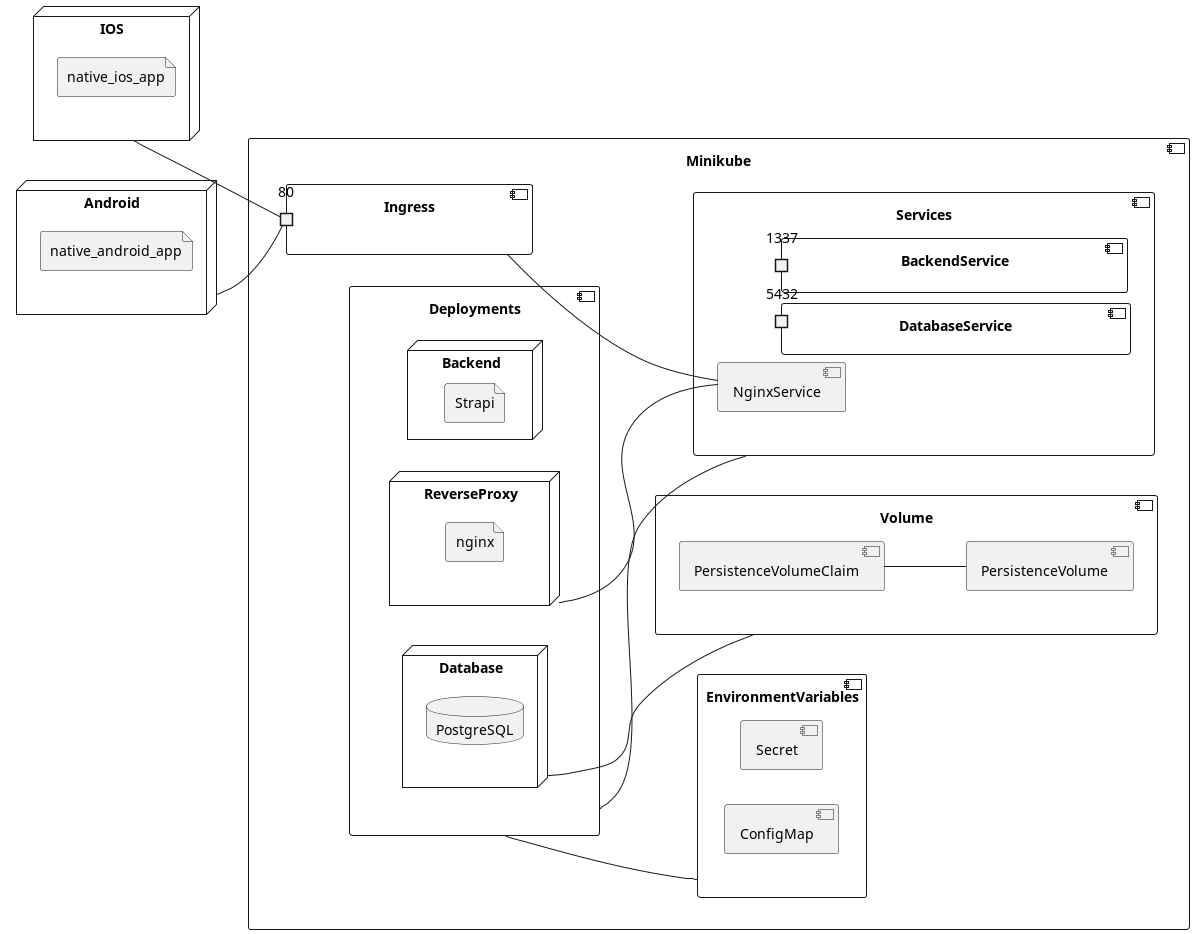
\includegraphics[width=\textwidth]{pics/dev-deployment.png}
\end{center}
\subsection{Deployment von dem Backend auf Minikube}

Damit ein funktionsfähiges Deployment erstellt werden kann sind diese Komponenten zu deployen:
\begin{itemize}
  \item Strapi
  \item Datenbank
\end{itemize}

Für jede dieser genannten Bauteile des Backends sind Kubernetes (K8S) Deployments und Kubernetes Services zu erstellen.

\subsection{K8S-Konfigurationen für die Datenbank}
Zusätzlich zu einer Deployment- und Service-Komponente ist für die Sicherung
von den Credentials der Datenbank eine sogenannte
Secret-Komponente gebraucht.
Für die Vermeidung von Datenverlusten in Fällen
wie Neustart eines Pods oder die Aktualisierung
der Konfiguration von dem Pod ist
das Anglegen einer PersistenceVolume-Komponente sehr dringend
Damit das Deployment auf die PersistenceVolume-Komponente zugreifen kann, ist eine sogenannte PersistenceVolumeClaim-Komponente zu definieren.

Für die Konfiguration der Secret-, Service- und Deployment-Komponente wurde die kubectl \textbf{C}ommand \textbf{L}ine \textbf{I}nterface verwendet
und für die PersistenceVolume-Komponente bzw. die PersistenceVolumeClaim-Kompoente wurden fertige Konfigurationen genommen.
\begin{lstlisting}[caption=K8S PVC]
  apiVersion: v1
  kind: PersistentVolumeClaim
  metadata:
    finalizers:
    - kubernetes.io/pvc-protection
    name: strapi-pvc
    namespace: default
  spec:
      accessModes:
        - ReadWriteMany
      resources:
        requests:
          storage: 10Mi
      storageClassName: standard
    
\end{lstlisting}


\begin{lstlisting}[caption=K8S PV]
  apiVersion: v1
  kind: PersistentVolume
  metadata:
    finalizers:
    - kubernetes.io/pv-protection
    labels:
      type: local
    name: strapi-volume
    resourceVersion: "33077"
    uid: ae6d772a-0090-4074-b3ac-1edb929daf29
  spec:
    accessModes:
    - ReadWriteOnce
    capacity:
      storage: 10Gi
    hostPath:
      path: /mnt/data
      type: ""
    persistentVolumeReclaimPolicy: Retain
    storageClassName: manual
    volumeMode: Filesystem
  status:
    phase: Available
    
\end{lstlisting}



\subsection{K8S-Konfigurationen für Strapi}
Für Strapi wird auch eine Secret-Komponente benötigt, da der Server geheime Umgebungsvariablen benötigt.
Es gibt auch einige.
Damit das Deployment von Strapi erstellt werden kann, muss die Anwendung zuerst in ein Docker Image umgewandelt werden. Dies kann mit der Verwendung des folgenden Dockerfiles erfolgen.
\begin{lstlisting}[caption=Strapi Dockerfile]
  # Creating multi-stage build for production
  FROM node:18-alpine as build
  RUN apk update && apk add --no-cache build-base gcc autoconf automake zlib-dev libpng-dev vips-dev git > /dev/null 2>&1
  ARG NODE_ENV=production
  ENV NODE_ENV=${NODE_ENV}
  
  WORKDIR /opt/
  COPY package.json package-lock.json ./
  RUN npm install -g node-gyp
  RUN npm config set fetch-retry-maxtimeout 600000 -g && npm install --only=production
  ENV PATH /opt/node_modules/.bin:$PATH
  WORKDIR /opt/app
  COPY . .
  RUN npm run build
  # Creating final production image
  FROM node:18-alpine
  RUN apk add --no-cache vips-dev
  ARG NODE_ENV=production
  ENV NODE_ENV=${NODE_ENV}
  ENV HOST=0.0.0.0
  ENV PORT=1337
  ENV APP_KEYS=secret
  ENV API_TOKEN_SALT=secret
  ENV ADMIN_JWT_SECRET=secret
  ENV TRANSFER_TOKEN_SALT=secret
  # Database
  
  # Database
  ENV DATABASE_CLIENT=postgres
  ENV DATABASE_HOST=localhost
  ENV DATABASE_PORT=5432
  ENV DATABASE_NAME=strapi
  ENV DATABASE_USERNAME=strapi
  ENV DATABASE_PASSWORD=strapi
  ENV DATABASE_SSL=false
  ENV JWT_SECRET=cVRog3q5woTNB8EJ+vKPFA==
  
  
  
  
  WORKDIR /opt/
  COPY --from=build /opt/node_modules ./node_modules
  WORKDIR /opt/app
  COPY --from=build /opt/app ./
  ENV PATH /opt/node_modules/.bin:$PATH
  
  RUN chown -R node:node /opt/app
  USER node
  EXPOSE 1337
  CMD ["npm", "run", "start"]
    
\end{lstlisting}

Dieses Image soll dann in einem Container Registry wie zum Beispiel
Dockerhub oder Github Container Registry hochgeladen werden,
damit die K8S-Deployment-Komponente dieses Image in Einsatz nimmt.




\subsection{K8S-Secrets}
Damit man Umgebungsvariablen in einem K8S-Cluster definieren kann gibt es zwei Möglichkeiten.
Man kann entweder eine ConfigMap-Komponente verwenden oder eine Secret-Komponente. Es gibt auch die Möglichkeit, diese Umgebungsvariablen direkt in den Konfigurationen von der Deployment-Komponente händisch einzutragen.
Für geheime bzw. sensible Daten werden K8S-Secrets verwendet.
Das Anlegen der benötigten Secrets für unsere Anwendung erfolgte durch die Verwendung folgender Befehle:
\begin{lstlisting}[caption=Secrets für Strapi]
    kubectl create secret generic strapi-server-secret \
  --from-literal=PORT=1337 \  
  --from-literal=APP_KEYS=secret
  --from-literal=API_TOKEN_SALT=secret \
  --from-literal=ADMIN_JWT_SECRET=secret \
  --from-literal=TRANSFER_TOKEN_SALT=secret \
  --from-literal=DATABASE_CLIENT=postgres \
  --from-literal=DATABASE_PORT=5432 \
  --from-literal=DATABASE_NAME=secret \
  --from-literal=DATABASE_USERNAME=secret \
  --from-literal=DATABASE_PASSWORD=secret \
  --from-literal=DATABASE_SSL=false \
  --from-literal=JWT_SECRET=secret
\end{lstlisting}


\begin{lstlisting}[caption=Secrets für die Datenbank]
kubectl create secret generic  strapi-secret \
--from-literal=POSTGRES_USER=strapi \
--from-literal=POSTGRES_PASSWORD=strapi \
--from-literal=POSTGRES_DB=strapi
\end{lstlisting}








\subsection{Was ist eine Deployment-Komponente}

Eine Deployment-Komponente dient dazu, dass ein Pod erstellt wird und die benötigten Resourcen bzw. Volumes und Zugriffsrechten
dafür definiert werden.\cite{k8s-deployment}

Für das Anlegen einer Deployment-Komponente muss man zuerst die Anwendung containerisieren.
Für weit verbreitete Software wie z.B.: PostgreSQL gibt es bereits viele vorhandene Images auf unterschiedliche Container-Registries.

Folgende Befehle wurden verwendet, um die Deployment-Komponenten für Strapi und PostgreSQL zu erstellen:

\begin{lstlisting}[language=bash, caption=create k8s deployments]
kubectl create deployment relaxoon-db --image=postgres:12.16-bullseye --port=5432
kubectl create deployment relaxoon-strapi --image=ghcr.io/Abdulrahman-AL-Sabagh/relaxoon-strapi:latest --port=8080
    
\end{lstlisting}


\subsubsection{Was ist ein Pod}

\begin{quotation}
  ``
  Ein Pod (übersetzt Gruppe/Schote, wie z. B. eine Gruppe von Walen oder eine Erbsenschote)
  ist eine Gruppe von einem oder mehreren Containern mit gemeinsam genutzten Speicher- und
  Netzwerkressourcen und einer Spezifikation für die Ausführung der Container.
  Die Ressourcen eines Pods befinden sich immer auf dem gleichen (virtuellen) Server,
  werden gemeinsam geplant und in einem gemeinsamen Kontext ausgeführt.
  Ein Pod modelliert einen anwendungsspezifischen ''logischen Server'': Er enthält eine oder mehrere
  containerisierte Anwendungen, die relativ stark voneinander abhängen.
  ''
  \cite{pod}
\end{quotation}






\subsection{Erstellung einer Service-Komponente}

Mit dem Einsatz eines Services in Kubernetes können Pods,
die sich im gleichen Cluster befinden, miteinander kommunizieren. \cite{k8s-service}

Für das Anlegen einer Service-Komponente kann man diesen Befehl nutzen:

\begin{lstlisting}[language=bash,caption=create a service component]
kubectl expose deployments/<Name des Pods> --port=5432
\end{lstlisting}






\subsection{Erstellung einer Ingress-Komponente}

Damit der Emulator, der sich außerhalb des lokalen Clusters von Minikube befindet,
mit dem deployten Backend kommunizieren kann,
ist das Anlegen einer Ingress notwendig.

//TODO Config für die Ingress-Komponente noch hingeben

//TODO Dieses Kapitel noch fertigschreiben



``
In einem Computernetzwerk befindet sich ein einfacher Reverse-Proxy zwischen einer
Gruppe von Servern und den Clients, die sie verwenden wollen.
Als Client gilt jede Hardware oder Software, die Anfragen an einen Server senden kann. [...].
Der Reverse-Proxy fängt alle Anfragen von den Clients an die Server ab und liefert auch
alle Antworten und Dienste von
en Servern wieder an die Clients zurück. Aus Sicht des Kunden sieht es so aus,
als würde alles von einer einzigen Stelle ausgehen.

''
\cite{reverse-proxy}

\subsection{Buildprozess für das Frontend}

Damit man das Frontend deployt, muss man zuerst den nativen Android und IOS Code generieren.
Danach sollen die Android bzw. IOS Anwendungen mit einer IDE oder mit der Kommando-Zeile gebaut werden.
Um den nativen Code zu generieren ist Folgendes einzugeben:
\begin{lstlisting}[language=Bash,caption=generate android and ios]
npx expo prebuild
\end{lstlisting}





\subsection{Erstellung einer .apk Datei}
Für Android wurde die .\textbf{A}ndroid \textbf{P}ac\textbf{K}age (apk)  mit dem Einsatz von gradle Wrapper generiert.
Folendes muss installiert und richtig konfiguriert werden, damit  eine .apk Datei generierbar ist:



\begin{itemize}
  \item Java 11
  \item Installation von sdkmanager
  \item Lizenzen von sdkmanager müssen akzeptiert sein
  \item Installation von einer Android SDK
  \item Konfigurationen für JAVA\_HOME und ANDROID\_HOME
  \item Installation einer CLI namens ''ninja''
\end{itemize}

Der Generierungsbefehl für die Build-Datei schaut dann wie folgendes aus:

\begin{lstlisting}[language=bash,caption=generate apk]
 ./gradlew assembleRelease
 \end{lstlisting}





\section{Hochladen einer Mobileapp auf Firebase App Distribution}

Nachdem Anlegen eines Accuonts bei Firebase sind folgende und die Erstellung eines Projektes Schritte zu machen:


\begin{figure}
  Damit die benötigten Firebase Services für die Applikationen aktiviert werden, muss man zuerst die benötigten Konfigurationen eingeben.
  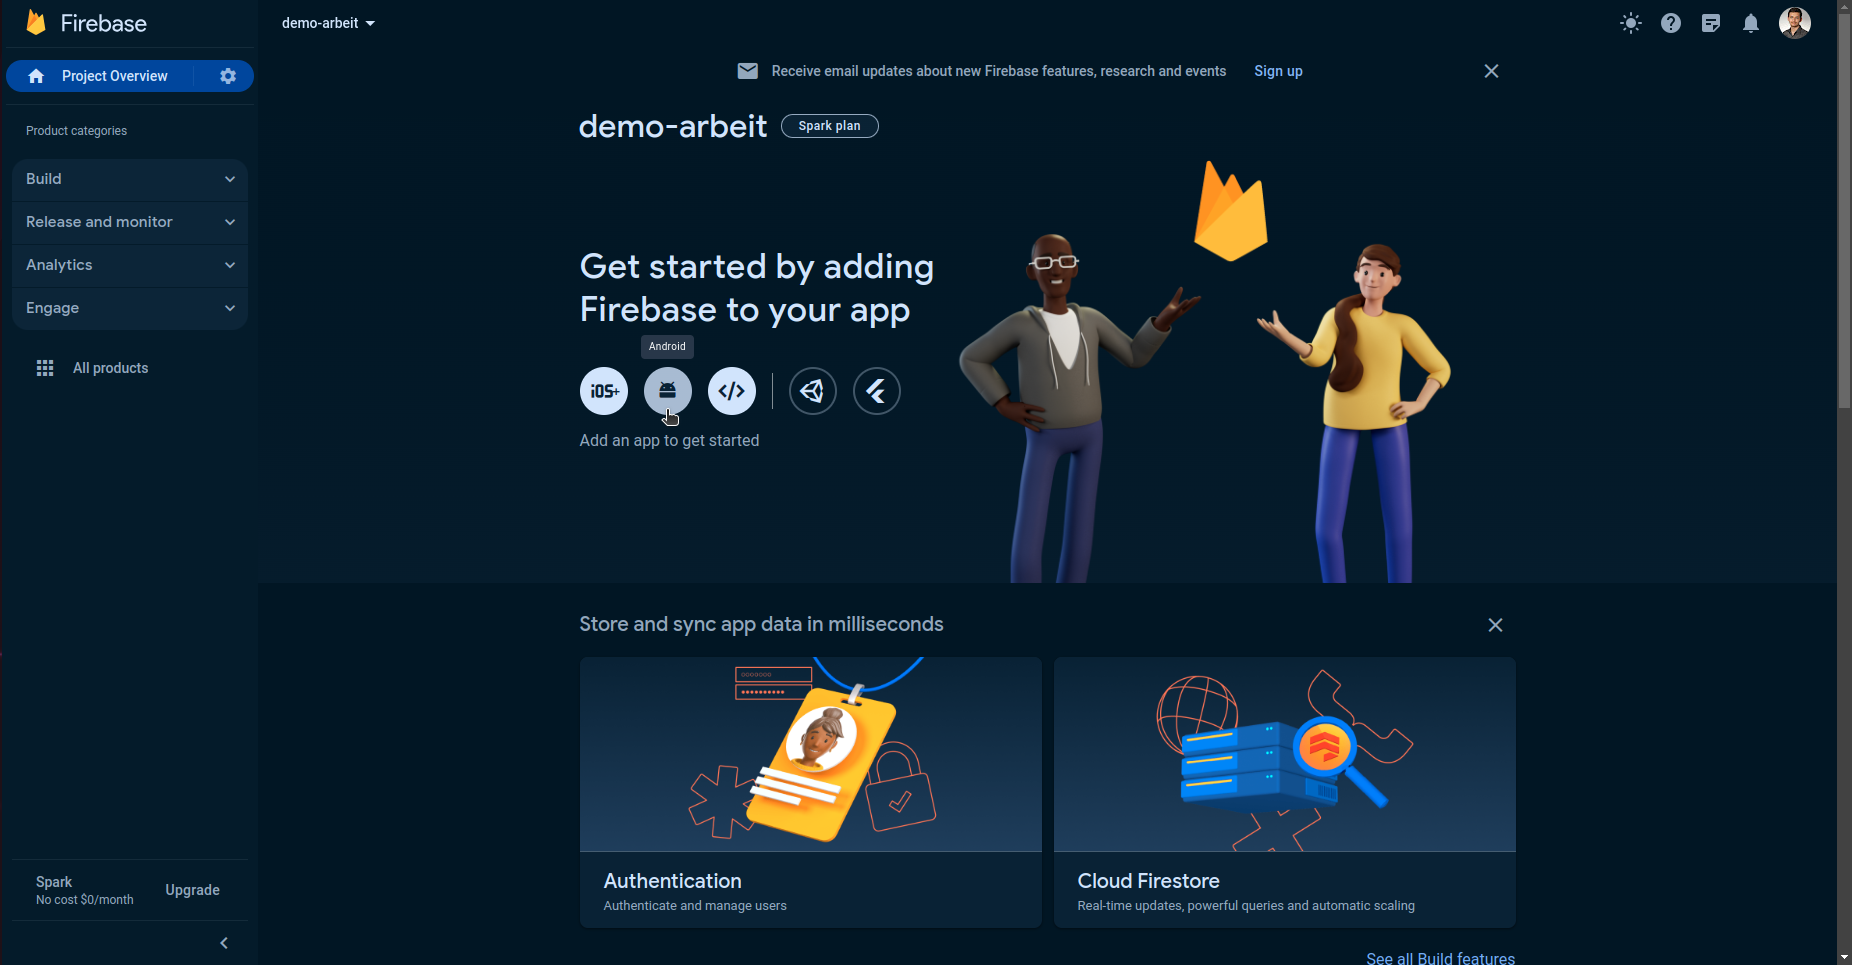
\includegraphics[width=\textwidth]{./pics/firebase1.png}
  \caption{create android config}
\end{figure}



\begin{figure}
  Folgende Daten müssen eingegeben werden, damit die Firebase Services für die Android Applikation eingeschaltet werden können.

  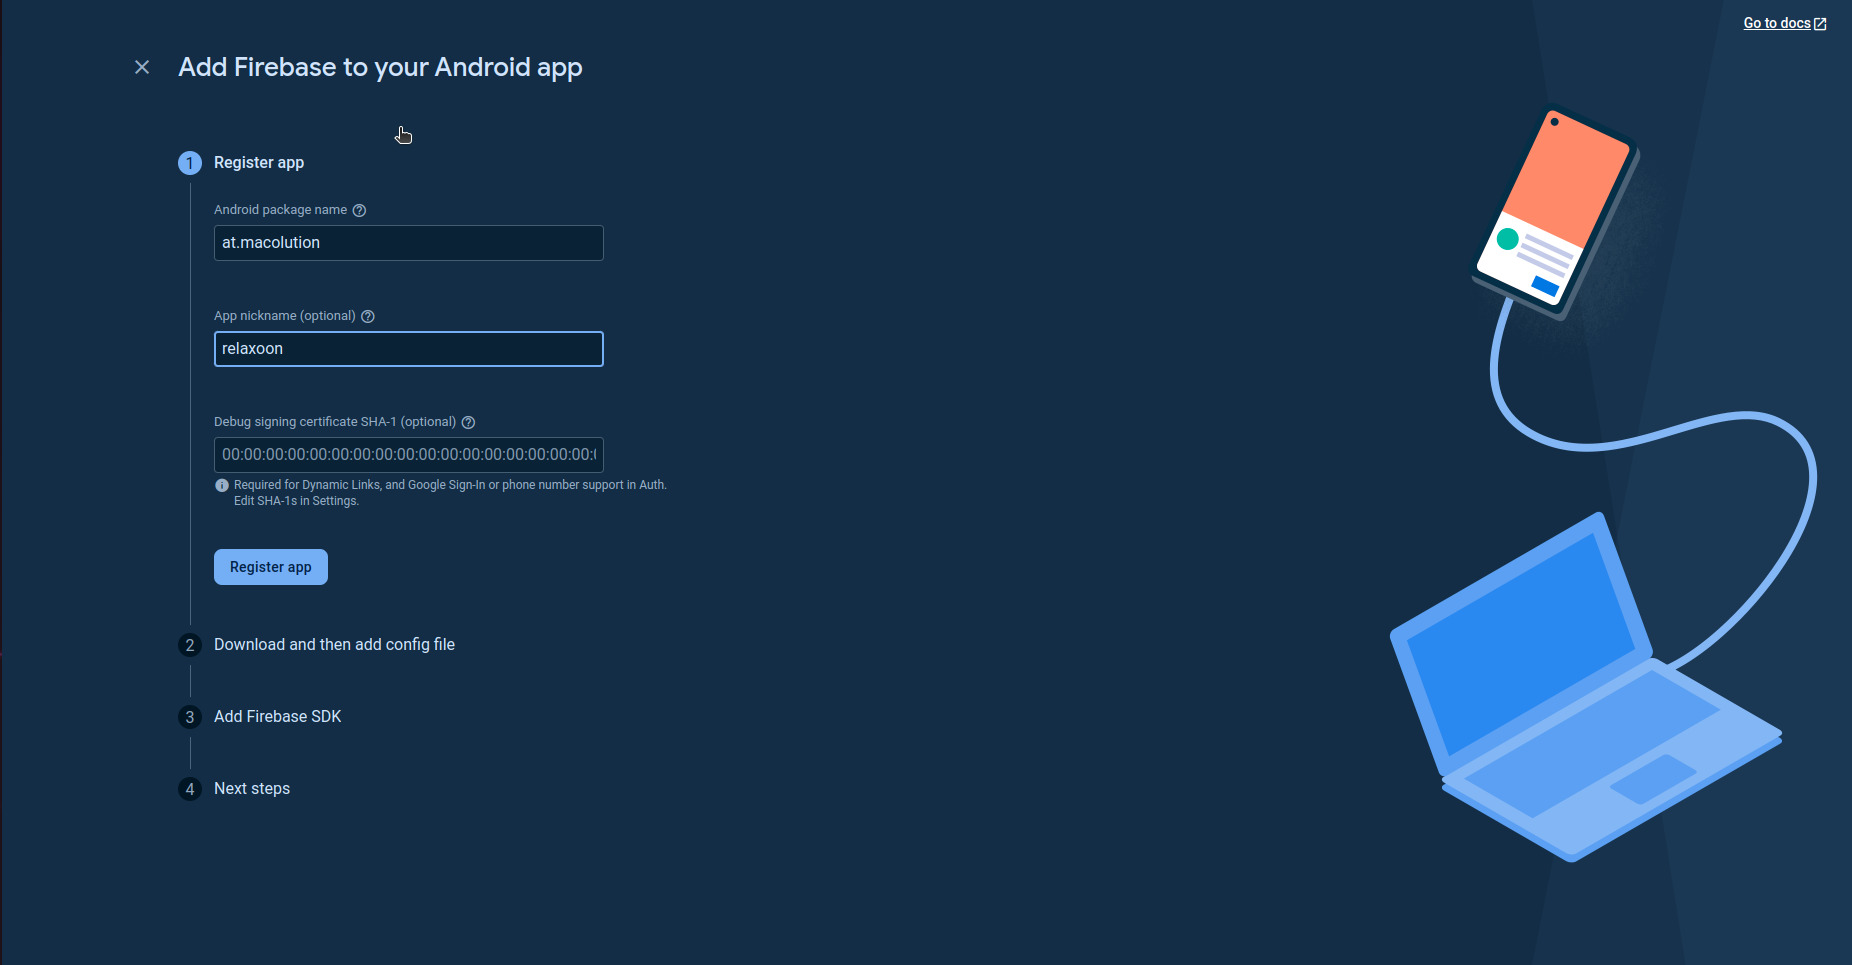
\includegraphics[width=\textwidth]{./pics/firebase2.png}
  \caption{Android Config}
  Die restlichen Punkte sind für das Projekt Relaxoon irrelevant,
  da die Firebase-SDK in der vorleigende Arbeit nicht eingesetzt wird.
\end{figure}



\begin{figure}
  Danach soll man  auf die App Distribution gehen und dann auf ''Get Started'' klicken
  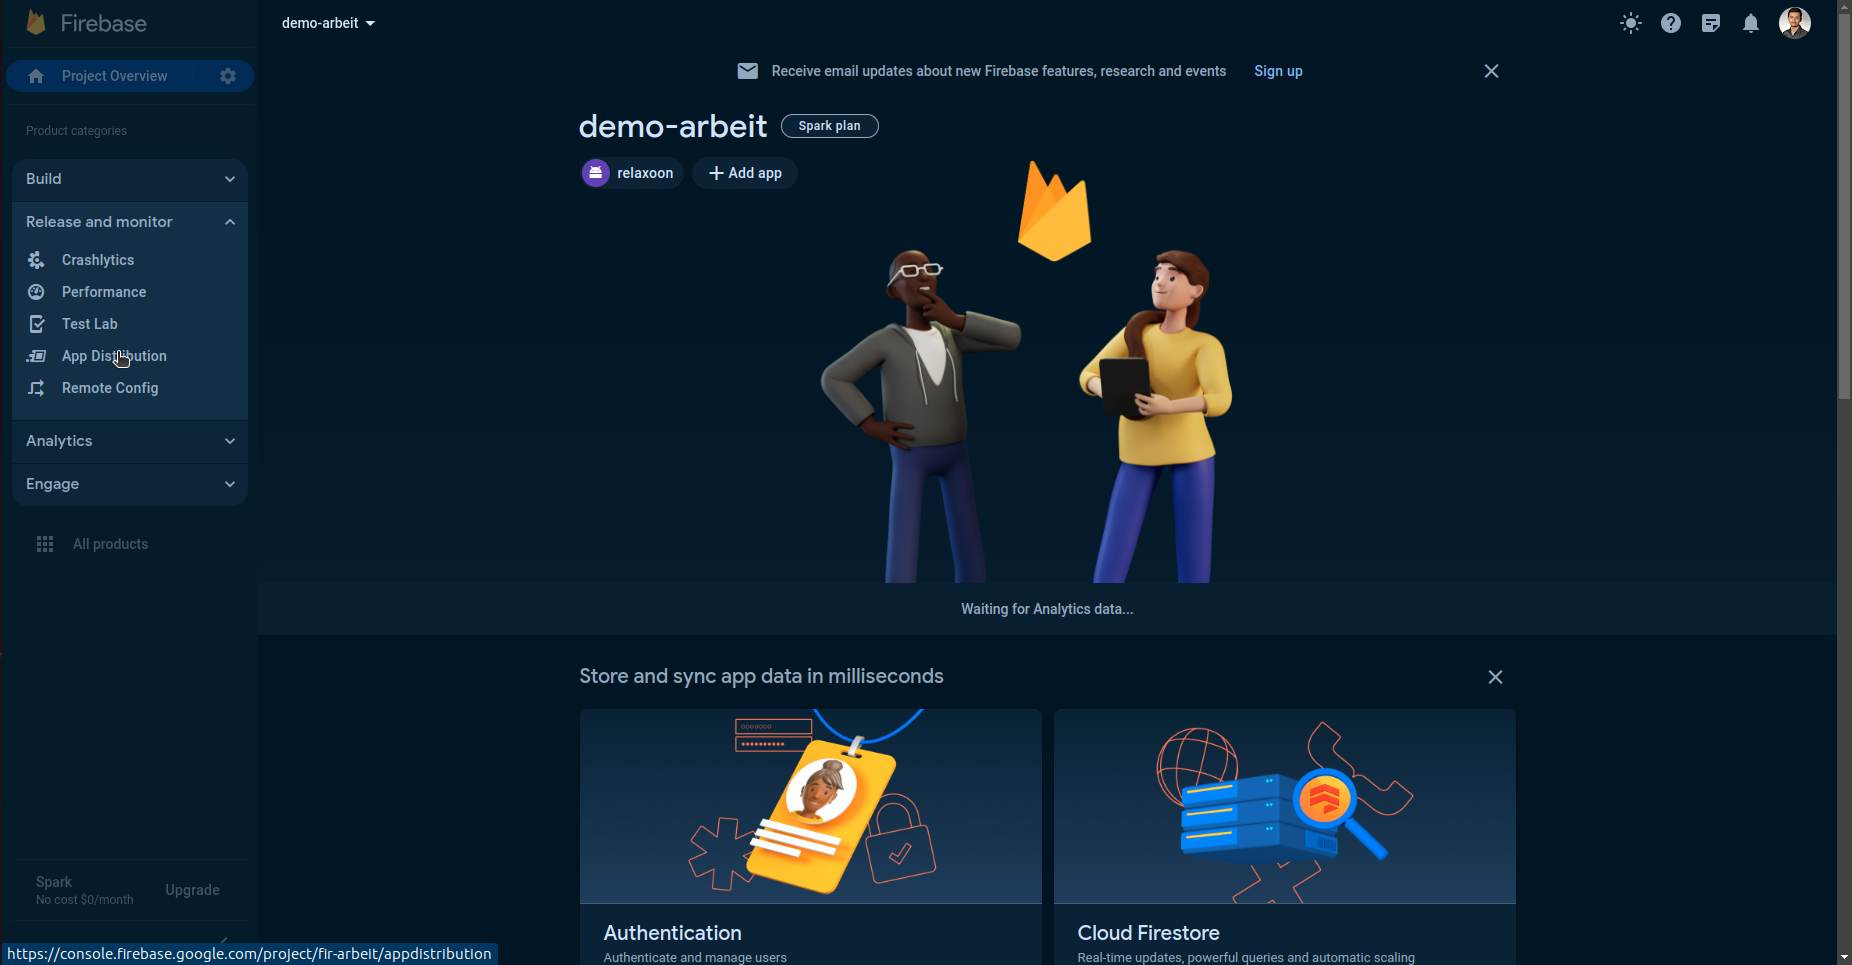
\includegraphics[width=\textwidth]{./pics/firebase3.png}
  \caption{App Distribution}
\end{figure}

\begin{figure}
  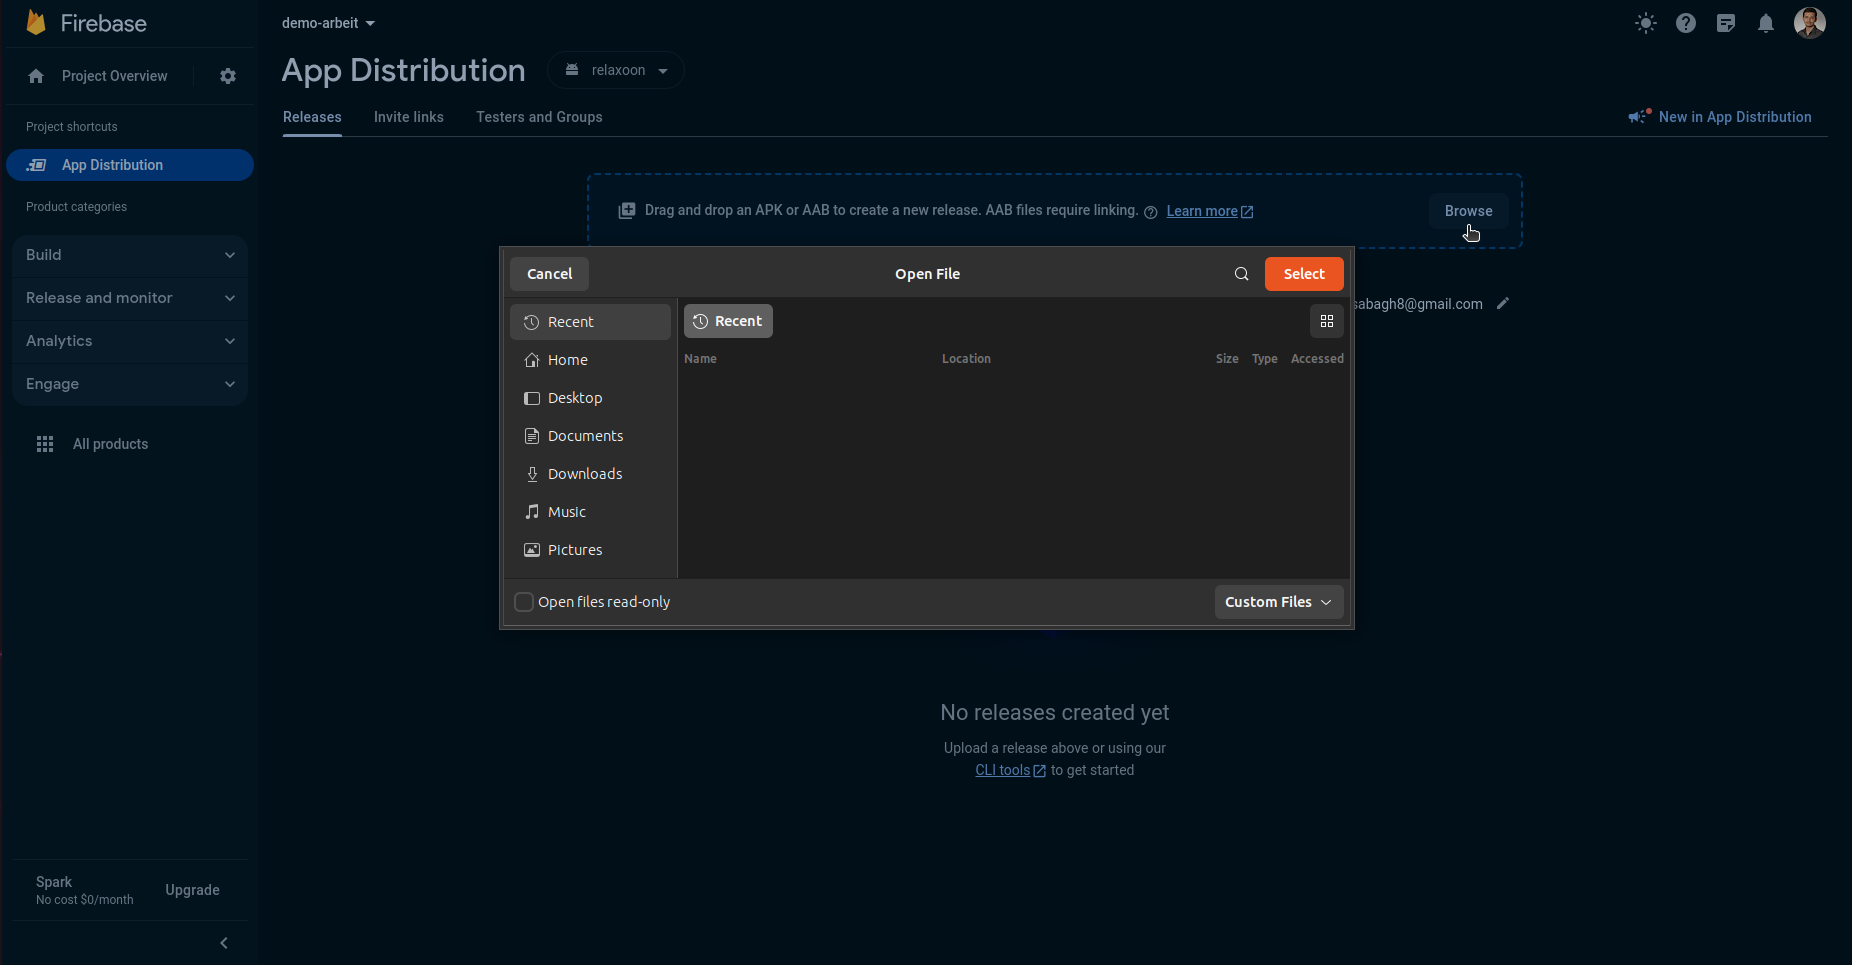
\includegraphics[width=\textwidth]{./pics/firebase4.png}
  \caption{App Upload}
  Die App kann mit diesem ''Browse Fenster'' oder mit ''Drag and Drop'' hochgeladen werden

\end{figure}



\begin{figure}
  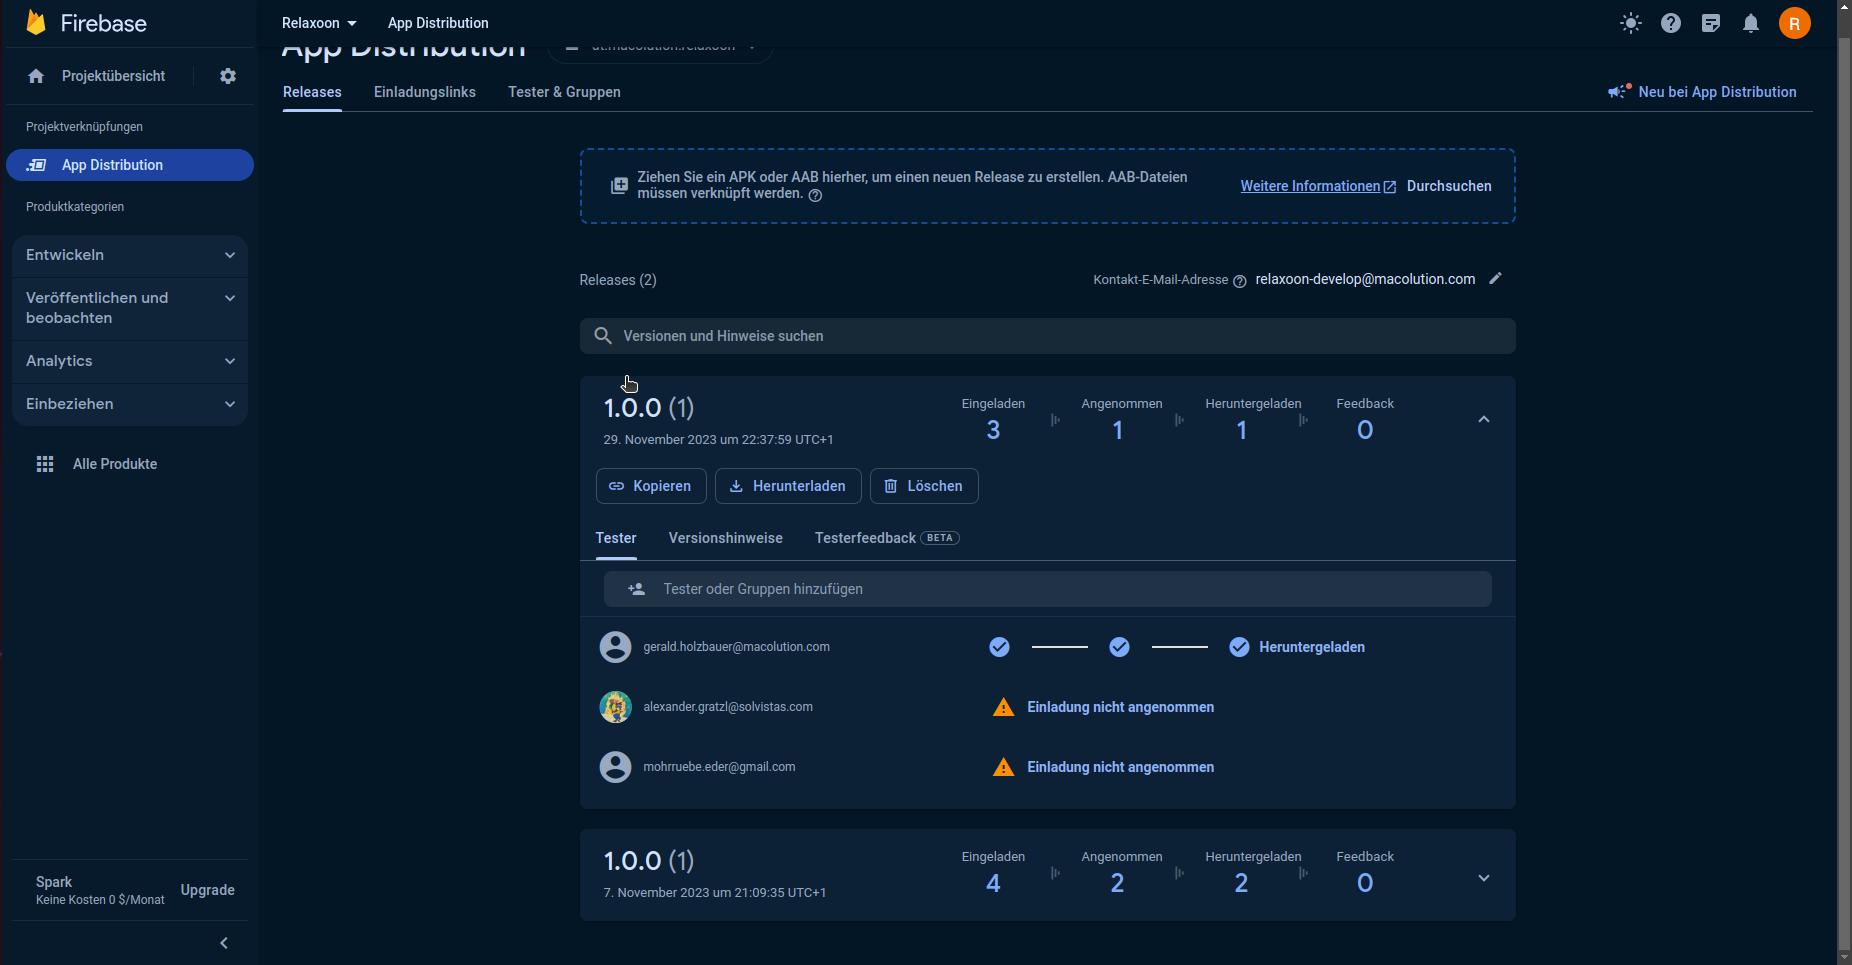
\includegraphics[width=\textwidth]{./pics/firebase5.png}
  \caption{Releases}
  
  Das Produkt kann dann an andere Testuser verteilt werden, indem man die Email-Adressen dieser 
  Tester beim Release eingibt.
\end{figure}






\begin{spacing}{1}
    \chapter{Ausgewählte Aspekte und Probleme}\label{chapter:probleme}
\end{spacing}
\setauthor{Abdulrahman Al Sabagh}
\begin{spacing}{1}


    \section{Probleme mit localhost und https}\label{sec:probleme-mit-localhost-und-https}

    Im Projekt wurde  die \textbf{U}niform \textbf{R}esource
    \textbf{L}ocater (URL) für den (API)-Server in einem ".env" File gespeichert.
    Für die lokale Entwicklung wurde Strapi auf dem lokalen Host immer verwendet.
    Bei IOS und Android ist das Holen der Daten von einer nicht sicheren Quellen
    \textbf{A}lso \textbf{K}nown \textbf{A}s (aka) nur http Protokolle gar nicht möglich. Auf Android gibt aber einige
    Ausnahmen für das Holen der Daten von dem lokalen Host
    Bei Android kann man bei den generierten Build und Project Files einige Konfigurationen ändern.
    Das ist zwar keine gute Lösung, da diese Files bei jedem Build geändert werden können.
    Außerdem können diese generierten Files nicht in das \textbf{V}ersion \textbf{C}ontrol \textbf{S}ystem (VCS)
    eingecheckt werden.
    Bei Android muss man 10.0.2.2 statt localhost schreiben.\cite{androidFetch}
    Bei IOS gibt es keine einzige Möglichkeit,
    um Daten aus http Quellen oder aus dem localhost zu holen.
    Als Lösung wurde in der lokalen Entwicklung eine \textbf{C}ommand \textbf{L}ine \textbf{I}nterface (CLI) namens "ngrok" verwendet,
    welche den lokalen Port des Servers ins Internet mittels eines Tunnels weiterleitet
    und eine https Adresse für den weitergeleiteten Server generiert.

    Das Problem tauchte wiederholt in der Test-Phase auf und war für die Entwickler nicht lösbar,
    da der Staging Server für das Backend von Relaxoon auf den Servern der Solvistas deployt ist.
    Die Entwickler verfügen über keine Zugriffsrechte auf diesem Server.
    Das Problem wurde mithilfe von den Netzwerkadministratoren von Solvistas gelöst.
    Es wurde ein "Let's encrypt" Zertifikat für den Staging Server eingebaut.





    \section{Inkompatible Libraries beim Build-Prozess}\label{sec:inkompatible-libraries-beim-build-prozess}
    In der Entwicklungsphase wurden einige Libraries mittels \textbf{N}ode  \textbf{P}ackage \textbf{M}anager (npm) installiert.
    Einige Libraries waren mit der Node Version oder mit anderen Libraries nicht kompatibel.
    Eine Lösung wäre, das Label "--legacy-peer-deps" oder "--force" beim Befehl "npm install" anzuhängen.
    Während der Entwicklung wurde das Label "--legacy-peer-deps" immer beim “npm install" integriert
    und danach hat alles problemlos funktioniert.
    Später beim Deployment von Android ist das Problem
    bei der Generierung von Android apk bzw.
    \textbf{A}ndroid \textbf{A}pp \textbf{B}undle (aab) aufgetaucht.
    Die Apk bzw.
    Aab wurde erfolgreich generiert, aber die App war nicht funktionsfähig.
    Es wurde für das Finden des Problems auf Android ein Tool namens “logcat” verwendet,
    um die Fehlermeldung zu finden.
    Dieses Problem an sich ist in der Community sehr stark verbreitet und es gibt dafür mehrere Gründe und mehrere Lösungen.
    Unter diesem Githublink \cite{libjsexecutor} werden unterschiedliche Gründe und mehrere
    Lösungsmöglichkeiten für das gleiche Problem beschrieben.
    Es wurde jede einzelne Lösungsmöglichkeit versucht und keine von diesen vorgeschlagenen Lösungen
    funktionierte.
    Aus Erfahrung hat man gewusst, dass der Codebase einige Libraries hat,
    die nicht mehr gebraucht bzw.
    verwendet werden. Beim Löschen dieser Libraries und die Wiederinstallation
    von den Modulen mittels "npm install" tauchte diese "legacy-peer-deps" Meldung wieder auf.
    Man dachte, dass das Problem daran liegt und es wurde  ein Tool namens "depcheck" installiert,
    welches den Codebase scannt und den Entwickler bekannt gibt, ob eine Library im Codebase verwendet
    wird oder nicht. \cite{depcheck}
    Nach dem Löschen aller nicht benötigten Libraries und die Generierung der
    apk bzw.
    aab hat die Applikation problemlos funktioniert.



    \subsection{npm install --legacy-peer-deps}\label{subsec:npm-install---legacy-peer-deps}
    \begin{quotation}
        ``
        The '--legacy-peer-deps' flag is used when you encounter compatibility issues with peer dependencies
        while installing packages.
        Peer dependencies are required by a package but aren't automatically
        installed alongside it.
        In some cases, when a package has not been updated to support the latest
        version of its peer dependency, the installation may fail due to conflicting versions.
        Adding the '--legacy-peer-deps' flag allows npm to use an older, compatible version of
        the peer dependency, ensuring a successful installation.''
        \cite{installFlags}
    \end{quotation}

    \subsection{npm install --force}\label{subsec:npm-install---force}
    \begin{quotation}
        ``
        The '--force'  flag is a more drastic option and should be used with caution.
        It instructs npm to forcefully install packages, even if it encounters errors or conflicts.
        This can be useful in situations where you want to override any version or compatibility checks
        and forcibly install packages.
        However, it is important to note that using '--force'
        may lead to unexpected issues, such as breaking dependencies or introducing incompatibilities,
        so it should be used sparingly and with a good understanding of its consequences.''
        ~\cite{installFlags}
    \end{quotation}



    \section{Probleme mit Thumbnails}\label{sec:probleme-mit-thumbnails}


    Unsere App soll mehrere Videos für Antistress-Meditationen anzeigen.
    Jedes Video muss unbedingt ein Thumbnail haben.
    Der Content-Manager könnte aber beim Erstellen des Videos vergessen,
    ein Thumbnail für das Video zu erstellen.
    Auf unserer Adminoberflächen können keine Thumbnails zu dem Video hinzugefügt werden,
    da diese Aktion sehr schlechte User Experience verursachen könnte.
    Man kann zwar eine Funktion implementieren,
    die nach dem Hochladen eines Videos ein Thumbnail mittels \textbf{F}ast \textbf{F}orward \textbf{M}oving
    \textbf{P}icture \textbf{E}xperts \textbf{G}roup (ffmpeg) aus dem ersten Bild des Videos erstellt.
    Diese Möglichkeit war aber sehr aufwendig und nicht empfehlenswert, da die damalige Dokumentation von
    Strapi nicht sehr genau war.
    Außerdem könnte diese Alternative bei den Updates von Dependencies nicht mehr funktionsfähig sein.
    Zum Glück haben wir eine Expo-Library gefunden, die im Frontend Thumbnails für unsere Videos erstellt.
    Die Verwendung davon war aber nicht sehr vorteilhaft, da der Generierungsprozess sehr langsam war.
    Als Lösung haben wir uns entschieden, ein nicht abspielbares Video auf den Screens, wo mehrere Videos vorgeschlagen werden,
    anzuzeigen.
    Das Video ist erst abspielbar, wenn man darauf klickt.
    Wir haben diese Lösung mit den Konzepten "Lazy Loading" und "Suspenses" zusammen kombiniert,
    damit Loading-Spinners statt leere Flächen für den User angezeigt werden,
    wenn das Laden des Videos etwas länger dauert.



    \subsection{Suspense}\label{subsec:suspense}

    \begin{quotation}

        ``<Suspense> lets you display a fallback until its children have finished
        loading.''~\cite{suspense}
    \end{quotation}

    \subsection{Lazy Loading}\label{subsec:lazy-loading}

    \begin{quotation}
        ``lazy lets you defer loading component’s code until it is rendered for
        the first time.''~\cite{lazyLoading}
    \end{quotation}


    \section{Dauer von Videos}\label{sec:dauer-von-videos}

    Beim Hochladen eines Videos in Strapi,
    wird die Dauer des Videos nur auf der Oberfläche angezeigt.
    Diese Information ist aber in den REST-Schnittstellen der Meta-Daten von den Files nicht inkludiert.
    Bei diesem Problem ist die Verwendung von ffmpeg auch eine Lösungsmöglichkeit.
    Es wurde aber nicht mit ffmpeg gearbeitet (siehe das obige Problem).
    Für die Berechnung der Dauers wurde im Frontend das "onLoad" Event,
    welches in den Properties (props) des Videoelements ist, verwendet,
    um die Dauer zu lesen und diese in das Format "mm:ss" umwandeln zu können.





    \section{Probleme mit useEffect und React-navigation Library}\label{sec:probleme-mit-useeffect-und-react-navigation-library}
    Für das Holen der Daten aus dem Server würde die Fetch API verwendet.
    Diese wurde auch in einem "useEffect Hook" eingegeben, damit die Daten bei jeder Aktualisierung eines spezifischen
    Zustandes aus dem Server geholt werden können.
    Beim Anklicken der unterschiedlichen Navigationsbuttons wurde bemerkt,
    dass die Daten sich gar nicht ändern.
    Am Anfang wurde vermutet, dass das Problem ein Caching Problem sein könnte.
    Nach einer Recherche kam man darauf, dass die Library "React-navigation" den "useEffect Hook" im Hintergrund deaktiviert.
    Für das Holen der Daten ist die Übergabe ein sogenanntes "useCallback Hook" als Parameter in einem custom hook namens "useFocusEffect"
    von React-navigation notwendig.\cite{issuesWithUseEffect}


    \subsection{Hooks}\label{subsec:hooks}
    \begin{quotation}
        ``Hooks let you use different React features from your components.
        You can either use the built-in Hooks or combine them to build your own.
        This page lists all built-in Hooks in React.''
        \cite{hooks}
    \end{quotation}

    \subsection{useEffect}\label{subsec:useeffect}
    \begin{quotation}
        ``useEffect is a React Hook that lets you synchronize a component
        with an external system.''~\cite{useEffect}

    \end{quotation}
    \begin{quotation}
        ``Some components need to synchronize with external systems.
        For example, you might want to control a non-React component based on the React state, set up a server connection,
        or send an analytics log when a component appears on the screen.
        Effects let you run some code after rendering so that you can synchronize your component with some system outside of React.[...]
        Effects let you specify side effects that are caused by rendering itself,
        rather than by a particular event. ''
        \cite{Synchronizing-with-effects}


    \end{quotation}


    \subsection{useCallback}\label{subsec:usecallback}
    \begin{quotation}
        ``useCallback is a React Hook that lets you cache a function definition between re-renders.''
        \cite{useCallback}
    \end{quotation}


    \subsection{useFocusEffect}\label{subsec:usefocuseffect}
    \begin{quotation}
        ``The useFocusEffect is analogous to React's useEffect hook. The only difference is that it only runs if the screen
        is currently focused.
        The effect will run whenever the dependencies passed to React.useCallback change,
        i.e. it'll run on initial render (if the screen is focused) as well as on subsequent renders if the dependencies
        have changed. If you don't wrap your effect in React.useCallback, the effect will run every render if the screen
        is focused.'' \cite{useFocusEffect}

    \end{quotation}


\end{spacing}




\begin{spacing}{1}
    \chapter{Resümee}
\end{spacing}
Aufzählungen:

\begin{compactitem}
    \item Itemize Level 1
    \begin{compactitem}
        \item Itemize Level 2
        \begin{compactitem}
            \item Itemize Level 3 (vermeiden)
        \end{compactitem}
    \end{compactitem}
\end{compactitem}

\begin{compactenum}
    \item Enumerate Level 1
    \begin{compactenum}
        \item Enumerate Level 2
        \begin{compactenum}
            \item Enumerate Level 3 (vermeiden)
        \end{compactenum}
    \end{compactenum}
\end{compactenum}

\begin{compactdesc}
    \item[Desc] Level 1
    \begin{compactdesc}
        \item[Desc] Level 2 (vermeiden)
        \begin{compactdesc}
            \item[Desc] Level 3 (vermeiden)
        \end{compactdesc}
    \end{compactdesc}
\end{compactdesc}

\newpage
\pagenumbering{Roman}
\setcounter{page}{\value{RPages}}
\newacronym{guid}{GUID}{Globally Unique Identifier}
\newacronym{jit}{JIT}{Just In Time Compiler}
\newacronym{nfc}{NFC}{Near Field Communication}
\newacronym{rfid}{RFID}{Radio Frequency Identification}

% Usage:
% \gls{label} lowercase in text
% \Gls{label} Uppercase in text
% \newacronym{label}{abbrev}{full}
% \newglossaryentry{label}{settings}



%\setlength{\glsdescwidth}{0.8\linewidth}
\glsnogroupskiptrue
\printglossary[title=Glossar,toctitle=Glossar] %,style=long]
\spacing{1}{
    %\bibliographystyle{IEEEtran}
    \bibliographystyle{ieeetrande}
    \bibliography{bib}
}
\listoffigures
\listoftables
\lstlistoflistings
\appendix
\addchap{Anhang}
\section{Prompt-Verlauf}

\textbf{Eingabe:} 

Erkläre mir den Unterschied zwischen funktionalen und nicht funktionalen Anforderungen.

\textbf{KI-Modell:} 

Funktionale und nicht-funktionale Anforderungen sind zwei Hauptkategorien von Anforderungen in der Softwareentwicklung und anderen Bereichen des Projektmanagements. Hier sind die grundlegenden Unterschiede zwischen ihnen:

Funktionale Anforderungen:
Beschreiben, welche Funktionen das System bereitstellen soll und welche Aufgaben es ausführen muss.
Definieren die spezifischen Funktionen, Dienste oder Aufgaben, die das System erfüllen muss, um die Benutzeranforderungen zu erfüllen.
Konzentrieren sich auf die "Was"-Aspekte des Systems und beschreiben, welche Ergebnisse erwartet werden.
Beispiel: "Das System muss dem Benutzer ermöglichen, sich mit einem Benutzernamen und Passwort anzumelden."

Nicht-funktionale Anforderungen:
Beschreiben Eigenschaften des Systems, die nicht unbedingt Funktionen sind, sondern Qualitätsmerkmale, die das System erfüllen muss.
Betreffen oft die "Wie"-Aspekte des Systems und definieren Qualitätsmerkmale wie Leistung, Sicherheit, Benutzerfreundlichkeit und Zuverlässigkeit.
Berücksichtigen Aspekte wie Skalierbarkeit, Wartbarkeit, Zuverlässigkeit, Leistung und Benutzerfreundlichkeit.
Beispiel: "Das System muss eine Antwortzeit von weniger als 2 Sekunden für Benutzeranfragen sicherstellen."

In einem Softwareprojekt sind funktionale Anforderungen eher auf die eigentlichen Aufgaben und Funktionen der Software ausgerichtet, während nicht-funktionale Anforderungen die Qualität und Leistung des Systems definieren. Beide Arten von Anforderungen sind wichtig, um ein vollständiges und erfolgreiches Produkt zu entwickeln, da sie gemeinsam die grundlegenden Spezifikationen und Erwartungen für das System festlegen.

%\rule{\linewidth}{0.5pt}

\section{Schriftliche Arbeitsaufteilung}

\begin{enumerate}
    \item Inhaltsverzeichniss
    \item Ausgangssituation [ME]
    \item Problemstellung [ME]
    \item Ziele [ME]
    \item Aufgabenstellung [ME]
    \item Marktanalyse [ME]
    \item Projektanforderungen [ME]
    \item Technologien [AA]
    \item Systemarchitektur [AA]
    \item Entwurfsentscheidungen [AA]
    \item Design [ME]
    \item Implementierung [AA]
    \item Ausgewählte Aspekte und Probleme [AA]
          \begin{enumerate}
              \item Relaxoon Plakat [ME]
          \end{enumerate}
    \item Resümee [ME]
\end{enumerate}
\newpage
\pagenumbering{Roman}
\end{document}

